\documentclass[12pt,letterpaper, oneside]{book}
\usepackage[ruled,vlined]{algorithm2e}
\usepackage{tabularx}
\usepackage{longtable}
\usepackage[utf8]{inputenc}
\usepackage[T1]{fontenc}
\usepackage{changepage}
\usepackage{tgtermes} % times font
\usepackage[spanish,es-tabla, es-lcroman]{babel}
\usepackage{amsmath}
\usepackage{amsfonts}
\usepackage{amssymb}
\usepackage{listings}
\usepackage{graphicx}
\usepackage[document]{ragged2e}
\usepackage{subfig}
\usepackage{wasysym}
\usepackage{lscape}
\usepackage[colorlinks=true, linkcolor=black,
citecolor=black, urlcolor=black,hidelinks]{hyperref}
\usepackage{float}
\usepackage{booktabs}
\usepackage{setspace} %por si el titulo es mas largo y el interlineado
\usepackage{xcolor} %para darle color a las lineas del titulo.
\usepackage{lipsum} %crea texto ficticio del texto Lorem Ipsum
\usepackage[left=4cm,top=4cm,right=2.6cm,,bottom=2.6cm]{geometry}
\usepackage[justification=centering]{caption}
\usepackage{svg}
\usepackage{hyperref}
\usepackage{adjustbox}

\captionsetup{belowskip=0pt}
% \onehalfspacing

\newcommand{\grad}{$^{\circ}$}
\renewcommand{\baselinestretch}{1.5} %interlineado 1.5

\usepackage{csquotes}
\usepackage[backend=biber,natbib,url=false,doi=false,style=apa,maxcitenames=5]{biblatex}

% Cuando el idioma es otro "et al." cambia, con este comando se fuerza a si o si usar "et al."
\DefineBibliographyStrings{spanish}{%
  andothers = {et\addabbrvspace al\adddot}
}
\addbibresource{chapters/biblio.bib}

\renewcommand{\labelenumii}{\arabic{enumi}.\arabic{enumii}}
\renewcommand{\labelenumiii}{\arabic{enumi}.\arabic{enumii}.\arabic{enumiii}}
\renewcommand{\labelenumiv}{\arabic{enumi}.\arabic{enumii}.\arabic{enumiii}.\arabic{enumiv}}

\definecolor{codegreen}{rgb}{0,0.6,0}
\definecolor{codegray}{rgb}{0.5,0.5,0.5}
\definecolor{codepurple}{rgb}{0.58,0,0.82}
\definecolor{backcolour}{rgb}{0.95,0.95,0.92}

\lstdefinestyle{mystyle}{
    backgroundcolor=\color{backcolour},   
    commentstyle=\color{codegreen},
    keywordstyle=\color{magenta},
    numberstyle=\tiny\color{codegray},
    stringstyle=\color{codepurple},
    basicstyle=\ttfamily\footnotesize,
    breakatwhitespace=false,         
    breaklines=true,                 
    captionpos=b,                    
    keepspaces=true,                 
    numbers=left,                    
    numbersep=5pt,                  
    showspaces=false,                
    showstringspaces=false,
    showtabs=false,                  
    tabsize=2
}
\lstset{style=mystyle}


% SE ELIMINA LA PALABRA "CAPÍTULO" DEL TÍTULO
\usepackage{titlesec}

% Capítulos sin la palabra "Capítulo "
\titleformat{\chapter}
  {\normalfont\normalsize\bfseries}{CAPÍTULO \thechapter}{0.5em}{}
%   \titlespacing*{\chapter}{0pt}{2pt}{2pt}
\titlespacing*{\chapter}{0pt}{0pt}{0pt}[0pt]
% \titlespacing*{\chapter}{0pt}{3.5ex plus 1ex minus .2ex}{2.3ex plus .2ex}

% Cambiamos el tamaño de las secciones
\titleformat{\section}
  {\normalfont\normalsize\bfseries}{\thesection.}{0.5em}{}
\titleformat{\subsection}
  {\normalfont\normalsize\bfseries}{\thesubsection.}{0.5em}{}

% SE ELIMINA LA CABECERA DE LAS HOJAS Y LA NUMERACIÓN ES ABAJO
\usepackage{fancyhdr}
\fancyhf{}
\renewcommand\headrulewidth{0pt}
% \fancyfoot[RO, LE]{\thepage}
% \fancyfoot[C]{\thepage}
% SE ENUMERA A LA DERECHA
\fancyfoot[R]{\thepage}
% SE REDEFINE EL ESTILO PARA ENUMERAR LAS PÁGINAS DE CAPÍTULO A LA DERECHA
\pagestyle{fancy}
\fancypagestyle{plain}{%
    \renewcommand{\headrulewidth}{0pt}%
    \fancyhf{}%
    \fancyfoot[R]{\thepage}%
}

% \renewcommand{\contentsname}{Índice}

\usepackage[subfigure]{tocloft}
% \setlength{\cftpartindent}{0em}
% \setlength{\cftchapindent}{0em}
\setlength{\cftsecindent}{0em}
\setlength{\cftsubsecindent}{0em}
\setlength{\cftsubsubsecindent}{0em}
% \setlength{\cftsubsubsecindent}{3em}

\usepackage{enumitem}
\setcounter{tocdepth}{4}
\setcounter{secnumdepth}{4}

\renewcommand*{\listalgorithmcfname}{ÍNDICE DE ALGORITMOS}
\renewcommand*{\algorithmcfname}{Algoritmo}
\renewcommand*{\algorithmautorefname}{algoritmo}
\SetKwInput{KwData}{Requiere}

\makeatletter
\patchcmd{\chapter}{\if@openright\cleardoublepage\else\clearpage\fi}{}{}{}
\makeatother

% Contar las figuras sin el capítulo
\usepackage{chngcntr}
\counterwithout{figure}{chapter}

\addto\captionsspanish{% Replace "spanish" with the language you use
  \renewcommand{\listalgorithmcfname}%
    {\fontsize{16}{20}\selectfont ÍNDICE DE ALGORITMOS}
}

% Editando el titulo del indice
\addto\captionsspanish{% Replace "spanish" with the language you use
  \renewcommand{\contentsname}%
    {\fontsize{16}{20}\selectfont ÍNDICE}
}
\addto\captionsspanish{% Replace "spanish" with the language you use
  \renewcommand{\listfigurename}%
    {\fontsize{16}{20}\selectfont ÍNDICE DE FIGURAS}
}

\addto\captionsspanish{% Replace "spanish" with the language you use
  \renewcommand{\listtablename}%
    {\fontsize{16}{20}\selectfont ÍNDICE DE TABLAS}
}
% quitando espacio del titulo del indice
\setlength{\cftbeforetoctitleskip}{-1em}
\setlength{\cftaftertoctitleskip}{1em}

% Quitando el identado en cada parrafo
\setlength\parindent{0pt}

% Espaciado entre parrafos
\setlength{\parskip}{0.5em}
\unaccentedoperators

\begin{document}
	%FRONTMATTER
	%---------------------------------------------------
	\frontmatter %numeros romanos
	\newgeometry{top=2.5cm, bottom=2.5cm, left=2.5cm, right=2.5cm}
\begin{titlepage} %este titlepage sirve para poder realizar el titulo de una pagina, la caratula de un libro y no se enumere esta.
	\begin{center}
	    {\fontsize{20}{20}\selectfont \textbf{UNIVERSIDAD MAYOR DE SAN ANDRÉS}}\\
		{\fontsize{16}{16}\selectfont \textbf{FACULTAD DE CIENCIAS PURAS Y NATURALES\\
		CARRERA DE INFORMÁTICA}}
		%\vspace{1mm}
		
		% 
\includegraphics[height=8cm]{images/logo_umsa.png}
		
\includegraphics[scale=0.20]{images/logo_umsa.png}
		%\vspace{1mm}
		
		{\fontsize{16}{20}\selectfont \textbf{TESIS DE GRADO}}\\
		%\vspace{2mm}
		
        {\fontsize{16}{18}\selectfont \textbf{COMPARACIÓN Y REFINAMIENTO DE ALGORITMOS DE FACTORIZACIÓN DE NÚMEROS ENTEROS}}
		
		{\fontsize{12}{12}\selectfont\textbf{Tesis de Grado para obtener el Título de Licenciatura en Informática Mención Ciencias de la Computación}}
 		%\vspace{2mm}
		
		{\fontsize{16}{16}\selectfont\textbf{POR: ROLANDO TROCHE VENEGAS}}\\
    	{\fontsize{14}{14}\selectfont\textbf{TUTOR: M.SC. JORGE HUMBERTO TERÁN POMIER}}
		%\vspace{2mm}
		 
		\textbf{LA PAZ - BOLIVIA\\
		2024}
	\end{center}
\end{titlepage}
\restoregeometry
	\chapter*{\centering \normalsize 
HOJA DE CALIFICACIONES\\
UNIVERSIDAD MAYOR DE SAN ANDRES\\
FACULTAD DE CIENCIAS PURAS Y NATURALES\\
CARRERA DE INFORMATICA\\ }
\begin{center}
    Tesis de Grado\\
    \textbf{COMPARACIÓN Y REFINAMIENTO DE ALGORITMOS DE FACTORIZACIÓN DE NÚMEROS ENTEROS}\\
\end{center}

% \doublespacing
\begin{flushleft}
Presentado por: Rolando Troche Venegas\\
Para optar por el grado academico de Licanciado en Informática\\
Mención Ciencias de la Computación\\

Nota Numeral: 95 \\
Nota Literal: Noventa y cinco \\
Ha sido: \\

Director de la carrera de Informática: Ph.D. Jose Maria Tapia Baltazar\\

\begin{tabular}{l l}
Tutor & M.Sc. Terán Pomier Jorge Humberto\\
Presidente & Lic. Carvajal Blanco Brigida Alexandra\\
Tribunal & M. Sc. Rodriguez Ramirez Grover Alex\\
Tribunal & P. Ph. D Cuenca Sarzuri Yohoni\\
\end{tabular}
\end{flushleft}

\newpage
\begin{figure}[h]
    \centering
    \begin{minipage}{0.1\textwidth}
        \begin{flushleft}
        
\includegraphics[width=1.5cm,height=3cm]{images/logo_umsa.png}
        \end{flushleft}
    \end{minipage}%
    \begin{minipage}{0.8\textwidth}
        \centering
        \textbf{
            UNIVERSIDAD MAYOR DE SAN ANDRES\\
            FACULTAD DE CIENCIAS PURAS Y NATURALES\\
            CARRERA DE INFORMATICA\\[1cm]
        }
    \end{minipage}%
    \begin{minipage}{0.1\textwidth}
        \begin{flushright}
        
\includegraphics[width=3cm,height=3cm]{images/logo_info.png} 
        \end{flushright}
    \end{minipage}
\end{figure}

\begin{justify}
    \textbf{
LA CARRERA DE INFORMÁTICA DE LA FACULTAD DE CIENCIAS PURAS Y NATURALES 
PERTENECIENTE A LA UNIVERSIDAD MAYOR DE SAN ANDRÉS AUTORIZA EL USO DE LA 
INFORMACIÓN CONTENIDA EN ESTE DOCUMENTO SI LOS 
PROPÓSITOS SON ESTRICTAMENTE ACADÉMICOS.
    }\\[1cm]
\end{justify}


\begin{center}
    \underline{\textbf{LICENCIA DE USO}}
\end{center}

\begin{flushleft}
    \textbf{El usuario está autorizado a:}

    
\end{flushleft}

\begin{enumerate}
    \item[a)] Visualizar el documento mediante el uso de un ordenador o dispositivo móvil

    \item[b)] copiar, almacenar o imprimir si ha de ser de uso exclusivamente personal y privado
    
    \item[c)] copiar textualmente parte(s) de su contenido mencionando la fuente y/o haciendo la referencia correspondiente respetando normas de redacción e investigación
\end{enumerate}

\begin{flushleft}
    El usuario no puede publicar, distribuir o realizar emisión o exhibición alguna de este material, sin la autorización correspondiente.\\[2cm]
\end{flushleft}


\begin{justify}
    TODOS LOS DERECHOS RESERVADOS. EL USO NO AUTORIZADO DE LOS CONTENIDOS PUBLICADOS EN ESTE SITIO DERIVARA EN EL INICIO DE ACCIONES LEGALES CONTEMPLADOS EN LA LEY DE DERECHOS DE AUTOR.
\end{justify}
  % \thispagestyle{empty}
% \vspace*{\fill}
\begin{adjustwidth}{4cm}{0cm}
  \begin{flushleft}
    \textbf{DEDICATORIA} \\
  \textit{Dedicado a mi familia, por creer en mí;\\
  a mis profesores, por iluminar el camino;}
  \end{flushleft}
\end{adjustwidth}
\vspace{2cm} 

  \clearpage

% \thispagestyle{empty} 

% \vspace*{\fill} 

\begin{flushleft}
\begin{center}
  \textbf{AGRADECIMIENTOS}
\end{center}

\textit{Quiero expresar mi más sincero agradecimiento a todos aquellos que me han brindado su apoyo y guía durante la elaboración de esta tesis: }\\
A mis padres, por su incondicional apoyo a lo largo de mi carrera y por ser mi fuente constante de inspiración y motivación. \\

A mi tutor, el M. Sc. Jorge Teran Pomier, por su invaluable apoyo, confianza y orientación durante todo el proceso de elaboración de esta tesis. \\

Al Club de Programación Competitiva U.M.S.A., por todo lo aprendido y las experiencias compartidas, las cuales han enriquecido mi formación y desarrollo profesional. \\

A mis amigos, "Los Osos", por ser los mejores compañeros que pude tener y por su compañía durante todo este camino en la universidad. \\ 

Finalmente, al lector, gracias por darle vida y sentido a este trabajo con su interés y atención. \\
% A mis padres por apoyarme a lo largo de mi carrera. \\
% A mi tutor M. Sc Jorge Teran Pomier por su apoyo y confianza en el proceso de elaboración
% de la presente tesis.\\
% Al Club de Programación Competitiva U.M.S.A. por todo lo aprendido y las experiencias que tuvimos.\\
% A los Osos, por ser los mejores amigos que pude tener y acompañarme durante este camino en la universidad. \\
% Al lector, gracias por darle vida y sentido a este trabajo.
\end{flushleft}

\vspace{\fill}
\begin{flushright}
  rtrochevenegas@gmail.com
\end{flushright}
  \clearpage
% \doublespacing
\chapter*{\centering \normalsize RESUMEN}
El teorema fundamental de la aritmética establece que todo número puede expresarse como un producto de números primos o ser un número primo. En matemáticas y, más recientemente, en ciencias de la computación, un problema de gran importancia es encontrar el conjunto de números primos que, al multiplicarse, nos den el número original. Esta propiedad fundamental no solo es interesante desde un punto de vista teórico, sino que también tiene aplicaciones prácticas significativas en diversas áreas de la ciencia y la tecnología.

Aunque desde la antigüedad se conocen algoritmos para realizar esta tarea, hoy en día cobra una relevancia particular debido a que gran parte de la seguridad informática se basa en la dificultad de factorizar números muy grandes. A pesar de que existen algoritmos eficientes y con complejidades polinomiales para esta tarea, el enorme tamaño de los números utilizados en la criptografía moderna hace que la factorización siga siendo un desafío considerable. Esta dificultad es precisamente la que garantiza la seguridad de muchos sistemas criptográficos, como RSA, que dependen de la factorización de números compuestos muy grandes.

En esta tesis se realizará un análisis y comparación de varios algoritmos y métodos de factorización para determinar cuáles son los más adecuados según el tipo de número y el contexto en el que se deben usar. Además, se abordará el refinamiento de estos métodos durante su implementación en un lenguaje de programación moderno. Se considerarán varios enfoques, desde los más clásicos como el método de la división por prueba hasta los más avanzados como el algoritmo de factorización de Lenstra basado en curvas elípticas y el método general de números.

La elección del algoritmo adecuado no solo depende del tamaño del número a factorizar, sino también de otros factores como la disponibilidad de recursos computacionales y el tiempo disponible para el proceso de factorización. Por ejemplo, para números relativamente pequeños, los métodos clásicos pueden ser suficientemente rápidos y eficientes. Sin embargo, para números extremadamente grandes, se requieren métodos más avanzados y sofisticados que aprovechen propiedades matemáticas más profundas y que puedan ser paralelizados en sistemas de computación distribuida.

Además de la comparación de algoritmos, esta tesis también explorará la implementación práctica de estos métodos. Se evaluará el rendimiento en un lenguaje de programación moderno. Se realizarán experimentos para medir el tiempo de ejecución y la eficiencia de los algoritmos implementados en Python.

% El teorema fundamental de la aritmética establece que todo número puede expresarse como un producto de números primos o ser un número primo. En matemáticas y, más recientemente, en ciencias de la computación, un problema de gran importancia es encontrar el conjunto de números primos que, al multiplicarse, nos den el número original.

% Aunque desde la antigüedad se conocen algoritmos para realizar esta tarea, hoy en día cobra una relevancia particular debido a que gran parte de la seguridad informática se basa en la dificultad de factorizar números muy grandes. A pesar de que existen algoritmos eficientes y con complejidades polinomiales para esta tarea, el enorme tamaño de los números utilizados en la criptografía moderna hace que la factorización siga siendo un desafío considerable.

% En esta tesis se realizará un análisis y comparación de varios algoritmos y métodos de factorización para determinar cuáles son los más adecuados según el tipo de número y el contexto en el que se deben usar. Además, se abordará el refinamiento de estos métodos durante su implementación en un lenguaje de programación moderno.\\
\textbf{Palabras clave:} Factorización, números primos, teorema fundamental de la aritmética, factores primos.

\clearpage
\chapter*{\centering \normalsize ABSTRACT}
The fundamental theorem of arithmetic states that every number can be expressed as a product of prime numbers or be a prime number. In mathematics and, more recently, in computer science, a problem of great importance is finding the set of prime numbers that, when multiplied, give us the original number. This fundamental property is not only interesting from a theoretical point of view, but also has significant practical applications in various areas of science and technology.

Although algorithms for this task have been known since ancient times, it is particularly relevant today because much of computer security is based on the difficulty of factoring very large numbers. Although efficient algorithms with polynomial complexity exist for this task, the enormous size of the numbers used in modern cryptography means that factorization remains a considerable challenge. This difficulty is precisely what guarantees the security of many cryptographic systems, such as RSA, which depend on the factorization of very large composite numbers.

This thesis will analyze and compare several factorization algorithms and methods to determine which ones are the most suitable for the type of number and the context in which they are to be used. In addition, the refinement of these methods during their implementation in a modern programming language will be addressed. Several approaches will be considered, from the most classical ones such as the trial division method to the most advanced ones such as the Lenstra factorization algorithm based on elliptic curves and the general number method.

The choice of the appropriate algorithm not only depends on the size of the number to be factored, but also on other factors such as the availability of computational resources and the time available for the factorization process. For example, for relatively small numbers, classical methods can be sufficiently fast and efficient. However, for extremely large numbers, more advanced and sophisticated methods are required that take advantage of deeper mathematical properties and that can be parallelized in distributed computing systems.

In addition to the comparison of algorithms, this thesis will also explore the practical implementation of these methods. Performance in a modern programming language will be evaluated. Experiments will be performed to measure the execution time and efficiency of the algorithms implemented in Python.
% The fundamental theorem of arithmetic states that every number can be expressed as a product of prime numbers or be a prime number. In mathematics and, more recently, in computer science, a problem of great importance is to find the set of prime numbers that, when multiplied, give us the original number.

% Although algorithms for this task have been known since ancient times, it is particularly relevant today because a large part of computer security is based on the difficulty of factoring very large numbers. Although efficient algorithms with polynomial complexity exist for this task, the enormous size of the numbers used in modern cryptography makes factorization still a considerable challenge.

% In this thesis, an analysis and comparison of various factorization algorithms and methods will be carried out to determine which are the most suitable according to the type of number and the context in which they must be used. In addition, the refinement of these methods during their implementation in a modern programming language will be addressed.\\
\textbf{Keywords:} Factorization, prime numbers, fundamental theorem of arithmetic, prime factors.


  % \singlespacing
	
	%ÍNDICE O TABLA DE CONTENIDO-------------------
	\tableofcontents
  \clearpage
  \listoffigures
  \clearpage
  \listoftables
  \clearpage
  \listofalgorithms
  \clearpage
	\setcounter{page}{1}
	%\cleardoublepage
% 	\addcontentsline{toc}{chapter}{Lista de figuras} % para 						que aparezca en el indice de contenidos
% 	\listoffigures % indice de figuras
	%\cleardoublepage
% 	\addcontentsline{toc}{chapter}{Lista de tablas} % para que 						aparezca en el indice de contenidos
% 	\listoftables % indice de tablas
	
	 % si no queremos que añada la palabra "Capitulo"
% 	\addcontentsline{toc}{chapter}{INTRODUCCIÓN} % si queremos que aparezca en el índice
	%\markboth{AGRADECIMIENTOS}{AGRADECIMIENTOS} % encabezado
	
	%MAINMATTER
	%--------------------------------------------------	
	\mainmatter %numeros arabicos.
    
    % \begingroup
    % \renewcommand{\cleardoublepage}{}
    % \renewcommand{\clearpage}{}
    
    \raggedbottom
    
    % \thispagestyle{empty}
    \chapter{ANTECEDENTES GENERALES O MARCO REFERENCIAL}
    \section{INTRODUCCIÓN}

    % \thispagestyle{empty}

    Factorizar números enteros es importante, hoy más que nunca la factorización de números enteros juega un papel crucial en la vida de todas las personas. Los métodos de encriptación actuales se basan, en gran medida, en la complejidad y el tiempo que toma factorizar números grandes.

    También se debe notar la definición de número grande, si se le pregunta a un niño que es un número grande este puede decirnos que es el 100 o hasta el 1000 y si se le preguntara a una persona adulta esta podría decirnos 1 000 000 o 100 000 000, pero esto no es nada si se piensa en los problemas que hoy en día lidian los matemáticos.

    Factorizar un número se refiere a encontrar todos los factores primos por los que está compuesto dicho número. El teorema fundamental de la aritmética nos dice que para todo número entero positivo mayor a 1 es un numero primo o bien un único producto de números primos (Euclides, 300 AC).
    \[
    n = \prod_{i=1}^{k}p_{i}^{a_{i}}
    \]
    Este es el objetivo que buscamos, encontrar esos factores para números, ahora sí, grandes.

    Los algoritmos de encriptación actuales, como RSA, usan números de, por ejemplo, 250 dígitos (829 bits) que fue el último en ser factorizado febrero de 2020. Estos son los números grandes que nos interesan. Los números RSA por ejemplo son números con exactamente dos factores primos, estos números primos, de al menos, la mitad de cantidad de dígitos que el resultado.

    Hoy en día tenemos diferentes métodos de factorización como los algoritmos simples de factorización, fracciones continuas, curva elíptica, algoritmos de cribado y hasta nuevos algoritmos basados en programación cuántica.

    En este trabajo se estudiará los diferentes métodos de factorización de números y su implementación con diferentes enfoques y refinamientos de implementación que el autor propondrá para ciertos métodos. Con esto se podrá revisar los alcances de los algoritmos de encriptación actuales y a donde se puede llegar en base a estos y realizar una comparación de los mismo, mostrando que algoritmo es el adecuado dada ciertas condiciones.
    \section{PROBLEMA}
        \subsection{ANTECEDENTES}
        Los algoritmos de factorización de números enteros han sido y son un area de interés en el campo de la teoría de números, criptografía y ciencias de la computación, los primeros algoritmos para realizar esta tarea sn tan antiguos como la matemática misma y con el pasar de los años se fueron agregando nuevos y mejores algoritmos y métodos para factorizar números enteros.

        Las siguientes investigaciones proporcionan un marco importante para el estudio de los algoritmos de factorización de números y han influido significativamente en el desarrollo de este campo:

        \begin{itemize}
            \item \textbf{Título:} ``A monte carlo method for factorization'' \\
            \textbf{Autor:} J. M. Pollard \\
            \textbf{Año:} 1975 \\
            \textbf{Institución:} BIT Numerical Mathematics \\
            \textbf{Resumen:} Se describe brevemente un nuevo método de factorización que involucra ideas probabilísticas y se sugiere que este método debería considerarse como una alternativa viable a los métodos de factorización tradicionales. \citep{Pollard1975}.
        
            \item \textbf{Título:} ``Theorems on factorization and primality testing'' \\
            \textbf{Autor:} J. M. Pollard \\
            \textbf{Año:} 1974 \\
            \textbf{Institución:} Mathematical Proceedings of the Cambridge Philosophical Society \\
            \textbf{Resumen:} Este artículo trata del problema de obtener estimaciones teóricas para el número de operaciones aritméticas necesarias para factorizar un entero grande $n$ o comprobar su primalidad. \citep{Pollard1974}.
        
            \item \textbf{Título:} ``A one line factoring algorithm'' \\
            \textbf{Autor:} W. B. Hart \\
            \textbf{Año:} 2012 \\
            \textbf{Institución:} Journal of the Australian Mathematical Society \\
            \textbf{Resumen:} Describimos una variante del algoritmo de factorización de Fermat que es competitiva con SQUFOF en la práctica, pero tiene una complejidad de tiempo de ejecución heurística $O(n^{1/3})$ como algoritmo de factorización general. También describimos una clase dispersa de números enteros para los que el algoritmo es particularmente eficaz. Ofrecemos comparaciones de velocidad entre una implementación optimizada del algoritmo descrito y la variedad optimizada de algoritmos de factorización en el paquete de álgebra computacional Pari/GP. \citep{Hart2012}.

            \item \textbf{Título:} ``A method of factoring and the
            factorization of F7'' \\
            \textbf{Autor:} M. A. Morrison and J. Brillhar\\
            \textbf{Año:} 1975 \\
            \textbf{Institución:} Mathematics of Computation, \\
            \textbf{Resumen:} Se analiza el método de fracciones continuas para factorizar números enteros, introducido por D. H. Lehmer y R. E. Powers, junto con su implementación informática. La potencia del método se demuestra con la factorización del séptimo número de Fermât $F_7$ y otros grandes números de interés. \citep{Morrison1975}.
        \end{itemize}
    
        \subsection{PLANTEAMIENTO DEL PROBLEMA}
        Con el avance de las computadoras y el mayor poder de cómputo, toda la seguridad basada en factorización y factores primos corre riesgo de quedar deprecada algún día.

        Por esto es necesario tener un compendio de gran parte de los métodos y algoritmos de factorización existentes y sus limitaciones, con el poder de cómputo actual. Por otro lado, hoy en día con la ayuda de los nuevos y mejores procesadores muchos algoritmos pueden ser paralelizados lo que reduciría su tiempo de ejecución.

        \subsection{FORMULACIÓN DEL PROBLEMA}
        ¿Qué método de factorización de números enteros es mejor de acuerdo a las características de los números?
    
    \section{OBJETIVOS}
        \subsection{OBJETIVO GENERAL}
        Estudiar y realizar una evaluación de números enteros con diferentes características y aplicando sobre ellos algoritmos de factorización de números enteros, comparando el tiempo de ejecución, espacio en memoria y factores primos encontrados.

        \subsection{OBJETIVOS ESPECÍFICOS}
        \begin{itemize}
            \item{Revisar el estado del arte referido a algoritmos de factorización de números enteros.}
            \item{Programar algoritmos de factorización de números enteros.}
            \item{Refinamiento de métodos de factorización de números enteros.}
            \item{Evaluar el desempeño de los programas con base en tiempo de ejecución, espacio en memoria y factores primos encontrados.}
        \end{itemize}
    
    \section{HIPÓTESIS}
    Para números donde la diferencia entre factores primos sea pequeña el algoritmo de Fermat es el mejor en cuanto a tiempo de ejecución, para números en general y de uso cotidiano el que presenta un mejor tiempo promedio es Pollard Rho y los métodos de cribado.
    
    \section{JUSTIFICACIÓN}
        \subsection{JUSTIFICACIÓN ECONÓMICA}
        Con el constante avance de la tecnología y la ciencia en diferentes campos hace que cada día se necesite de mejores equipos, maquinaria, software, hardware entre otros, lo cual implica costos gigantescos, por lo cual hacer una redefinición en las herramientas teóricas resulta ser un gran ahorro y reducción de gastos para las diferentes investigaciones realizadas por universidades, instituciones del estado, comunidades científicas.

        Además de una reducción de tiempos, el cual es representado a su vez en una reducción de costos, mejorando así la accesibilidad a nuevos campos de investigación.
        
        \subsection{JUSTIFICACIÓN SOCIAL}
        La sociedad en su conjunto se beneficia indirectamente ya que la presente investigación está enfocada al área teórica pero enteramente ligada a futuros campos de investigación y aplicación para mejorar el estilo de vida, hambre de conocimientos y experimentación por parte de la población en general.

        \subsection{JUSTIFICACIÓN CIENTÍFICA}
        La presente investigación brinda al campo científico tecnológico un complejo análisis de diferentes algoritmos de factorización, lo cual conlleva a tener nuevos y/o actualizaciones de los mismos generando avances en diferentes campos no solo del área sino también de otros campos afines, generando propuestas o aplicaciones de la presente investigación.

        Por lo tanto, al emprender la investigación de los algoritmos de factorización de números enteros grandes y su evaluación, profundiza el conocimiento, aportando así a futuras investigaciones, ya que se está trabajando en un área en desarrollo. Así también como bases prácticas y teóricas para la aplicación de dichos algoritmos en áreas como el análisis complejo de números primos, representación del conocimiento, teoría de números, criptografía, combinatoria, entre otros.
    
    \section{ALCANCES Y LIMITES}
        \subsection{ALCANCES}
        \begin{itemize}
            \item{Se implementaran los métodos teoricos descritos en un lenguage de programacion moderno.}
            \item{Se realizará un análisis teórico mediante una función que limitará el tiempo de cálculo del algoritmo y una prueba experimental de dónde se recogerán estadísticas de tiempo consumido por los diferentes algoritmos.}
            \item{Se refinara los métodos a nivel de implementacion.}
            \item{Se comparara los resultados de los diferentes tiempos de ejecucion y memoria de cada algoritmo}
            
        \end{itemize}
        \subsection{LIMITES}
        \begin{itemize}
            \item{No se tomara en cuenta algoritmos cuanticos.}
            \item{No se tomara en cuenta algoritmos hibridos.}
            \item{No se demostrara la correctitud de los métodos de manera teorica.}
        \end{itemize}
    
    \section{METODOLOGÍA}
    Para el desarrollo del presente trabajo se utilizará el método lógico inductivo ya que partiremos de casos particulares de factorización de números enteros para posteriormente llegar a una conclusión respecto a cada uno de los algoritmos que serán comparados y refinados.
    
    \clearpage
\chapter{MARCO TEÓRICO}
En el desarrollo de este capítulo se plantea la teoría relacionada con divisibilidad, números primos, factorización, congruencia, diferentes definiciones en teoría de números que serán fundamentales para el desarrollo de los posteriores algoritmos.
    
    \section{NÚMEROS ENTEROS}
    La teoría de números se ocupa de las propiedades de los números naturales $1, 2, 3, 4, \dots$, también llamados enteros positivos. Estos números, juntos con los enteros negativos y cero, forman el conjunto de números enteros \citep{NZM1991}.

    Para el desarrollo de las siguientes definiciones y algoritmos usaremos la notación de conjuntos para referirnos a los números naturales $ \mathbb{N} = {1, 2, 3,4, \dots}$ y números enteros $ \mathbb{Z} = \dots, -2, -1, 0, 1, 2, \dots$ y usualmente si se habla de “número” nos referiremos a un número entero.

    \section{DIVISIBILIDAD}
    Un entero $a$ se dice que es divisible por otro entero $b$, no $0$, si es que existe un tercer entero $c$ tal que $a=b\cdot c$
    Si $a$ y $b$ son positivos, $c$ es necesariamente positivo. Se expresa el echo de que $a$ es divisible por $b$, o $b$ es un divisor de $a$, con $b \mid a$
    Por lo tanto $1 \mid a$, $a \mid a$; y que $b \mid 0$ para cualquier $b$ excepto 0. También se puede decir que $b \nmid a$ para expresar lo contrario a $b \mid a$.
    Otras propiedades que podemos notar son:
    \begin{itemize}
        \item{$b \mid a \land c \mid b \implies c \mid a$}
        \item{$b \mid a \implies b\cdot c \mid a\cdot c$}
        \item{Si $c\not = 0$ y $c \mid a \land c \mid b \implies c\mid m\cdot a + n\cdot b$ para todos los enteros $m$ y $n$ }
    \end{itemize}
    \[
        b \mid a \land c \mid b \implies c \mid a
    \]

    \[
        b \mid a \implies b\cdot c \mid a\cdot c
    \]
    
    Si $c\not = 0$ y $c \mid a \land c \mid b \implies c\mid m\cdot a + n\cdot b$ para todos los enteros $m$ y $n$ \citep{HW1975}.

    Definimos “$n \mod m$” como el resto cuando el entero $n$ es divido por el entero positivo $m$. Siempre se tiene que $0 \leq n \mod m < m$.
    Si al menos uno de los enteros $n$, $m$ no es cero, se define el máximo común divisor (\textit{greatest common divisor}) de $n$ y $m$, como $gcd(m,n)$, al mayor entero que divida a ambos $m$ y $n$. Esta claro que $gcd(m,n) \geq 1$ y que $gcd(m,n) = gcd(n,m)$. Se dice que los enteros $m$, $n$ son primos relativos o coprimos si $gcd(m,n) = 1$ \citep{Wagstaff2013}.

    El siguiente enunciado es util para los algoritmos que usaremos más adelante, si $m$ es un entero positivo y $n$, $q$, $r$ son enteros tal que $n = m\cdot q + r$, entonces $gcd(n,m) = gcd(m,r)$ y su demostración es la siguiente:

    Si $a = gcd(n,m)$ y $b=gcd(m,r)$. Dado que $a$ divide a ambos $n$ y $m$, también debe dividir a $r =n-m\cdot q$. Esto muestra que $a$ es un común divisor de $m$ y $r$, entonces este debe ser $\leq b$, su máximo común divisor. Igualmente, dado que $b$ divide a ambos $m$ y $r$, este debe dividir a $n$, entonces $b \leq a = gcd(n,m)$. Por lo tanto $a = b$.

    \section{NOTACIÓN BIG-O}
    Para las funciones dadas $g(n)$, denotaremos por $O(g(n))$ (pronunciado como ''big-oh de g de n'' o solamente ''oh de g de n'') al conjunto de funciones
    \[
        O(g(n)) = \{ f(n):\text{si existe una constante positiva }c \text{ y }\text{ tal que } 0 \leq f(n) \leq c\cdot g(n)\}.
    \]
    Usaremos la notación Big O para dar un limite superior a una función, dentro de un factor constante \citep{Cormen2009}

    La notación Big O es una forma de describir el comportamiento de un algoritmo en términos de la cantidad de tiempo o espacio que necesita a medida que el tamaño de la entrada crece. Se utiliza principalmente en el análisis de algoritmos para medir su eficiencia y compararlos. La notación Big O se centra en el crecimiento asintótico del tiempo o espacio requerido, lo que significa que describe cómo se comporta el algoritmo cuando la entrada se vuelve muy grande.

    La notación Big O se centra en el peor caso, lo que proporciona una garantía sobre el comportamiento del algoritmo independientemente de las condiciones específicas de la entrada

    \section{ALGORITMO DE EUCLIDES}
    El algoritmo de Euclides es el algoritmo eficiente más antiguo que se tiene, se lo usa desde hace 2500 años, descrito por primera vez por Euclides en su obra Elementos.

    Para computar $gcd(m,n)$, con $m\geq n > 0$, el algoritmo repetidamente remplaza el par $(m,n)$ por el par $(n, m \mod n)$ hasta $n=0$, en ese punto m es el máximo común divisor que se buscaba.
    
    \begin{algorithm}[H]
        \SetAlgoLined
        \textbf{Entrada:} Enteros $m >= n > 0$ \;
         \While{$n > 0$}{
          $r \leftarrow m$ mod $n$\;
          $m \leftarrow n$\;
          $n \leftarrow r$\;
         }
         \textbf{Salida:} $gcd(m,n)=$ el valor final de $m$.\ 
         \caption{Algoritmo de Euclides}
    \end{algorithm}

    \section{ALGORITMO EXTENDIDO DE EUCLIDES}
    Si $m$ y $n$ son enteros y al menos uno de ellos no es $0$, entonces existen enteros $x$ y $y$ tales que $m\cdot x + n\cdot x = gcd(m, n)$
    Esto es importante para calcular el inverso modular $m$ y para calcular estos valores $x$, y se puede usar el algoritmo extendido de Euclides.
    Para el siguiente algoritmo se usara tripletas de enteros, como $u = (u_{0}, u_{1}, u_{2})$, las cuales son sumadas y multiplicadas por enteros usando las reglas de suma vectorial y multiplicación escalar.

    \begin{algorithm}[H]
        \SetAlgoLined
        \textbf{Entrada:} Enteros $m >= n > 0$ \;
        $\vec{u} \leftarrow (m,1,0)$\;
        $\vec{v} \leftarrow (n,0,1)$\;
         \While{$v_0 > 0$}{
          $q \leftarrow \lfloor u_0 / v_0 \rfloor$\;
          $\vec{w} \leftarrow \vec{u} - q\vec{v}$\;
          $\vec{u} \leftarrow \vec{v}$\;
          $\vec{v} \leftarrow \vec{w}$\;
         }
         \textbf{Salida:} $(gcd(m,n),x,y)=$ el valor final de $\vec{u}$.\ 
         \caption{Algoritmo extendido de Euclides}
    \end{algorithm}

    Los números $x$ y $y$ no son únicos, pero el algoritmo retorna los $x$ y $y$ con valor absoluto más pequeños. El algoritmo funciona porque cada tripleta $(a,b,c)$ satisface $a = b\cdot m + c\cdot n$ durante el algoritmo.

    \section{NÚMEROS PRIMOS}
    Un entero $p > 1$ es llamado número primo, o simplemente primo, si no existe un divisor $d$ de $p$ que satisfaga $1 < d < p$. Si un entero $a > 1$ no es un primo, es llamado un número compuesto.

    \section{TEOREMA FUNDAMENTAL DE LA ARITMÉTICA}
    Todos los enteros mayores a $1$ se pueden escribir como un producto de primos, este producto es único aparte del orden de los factores primos, y a este producto se llamara la factorización de dicho numero.
    \[
        n = p_{1} \times p_{2} \times p_{3} \times p_{4}
    \]
    Si se tiene $e$ copias de un primo $p_{i}$ en el producto, este se puede reescribir como $p_{i}^{e}$, de esta forma se obtiene la forma canónica de la factorización de un entero $n$ como:
    \[
        n = \prod_{i=1}^{k}p_{i}^{e_{i}}
    \]
    donde $p_{1}, p_{2},\dots, p_{k}$ son los distintos primos que dividen a $n$ y $e_{i} \geq 1$ es el número de veces que $p_{i}$ divide a $n$. Si $n$ es primo, solo existe un “factor”, el mismo primo. También esta permitido $n=1$ con el “producto vació” para esta forma canónica.
    
    \section{CONGRUENCIA}
    Si $m$ es un entero positivo y, $a$ y $b$ son enteros, se puede decir a que $a$ es congruente con $b$ módulo $m$ y escribir $a = b(\mod m)$ si $m$ divide a $a-b$. Si $m \nmid (a-b)$ se escribe $a \not = b(\mod m)$. El entero $m$ es llamado el módulo. Cuando $a = b (\mod m)$, cada uno $a$ y $b$ son llamados residuos del otro (modulo $m$). Congruencia modulo $m$ es una relación de equivalencia, lo que significa que si $a$, $b$ y $c$ son enteros, entonces:
    
    \begin{itemize}
        \item{$a = a \mod m$}
        \item{Si $a = b \mod m$, entonces $b = a \mod m$}
        \item{Si $a = b \mod m$ y $b = c \mod m$ entonces $a = c \mod m$}
    \end{itemize}
    La congruencia $a = b \mod m$ es equivalente a decir que existe un entero $k$ tal que $a = b + k\cdot m$.

    % \section{NOTACIÓN BIG O}
    \section{DIVISIONES SUCESIVAS}
    Si se quiere encontrar los factores primos de $n$ lo que se hace es tener una lista de todos los números primos menores a $n$, luego se prueba dividir  entre cada primo $p_{i}$, si $p_{i} \mid n$ entonces se vuelve a hacer el proceso desde ese primo, pero ahora con $n/p$. Si se llega a $\sqrt{n}$ y no se ha encontrado ningún primo que divida a $n$, entonces se declara a $n$ como primo. \citep{Knuth1976}

    \section{MÉTODO DE DIFERENCIA DE CUADRADOS DE FERMAT}
    Para factorizar un número impar $n$, Fermat trato de expresar $n$ como una diferencia de dos cuadrados, $x^{2}-y^{2}$ con el par $x$, $y$ diferente de $\frac{n+1}{2}$, $\frac{n-1}{2}$. Este par entrega $x + y = n$ y $x - y =1$. Cualquier otra representación de $n$ como $x^{2}-y^{2}$ entrega una factorización no trivial $n = (x - y)\cdot (x + y)$. \citep{Fermat1894}

    \begin{algorithm}[H]
        \SetAlgoLined
        \textbf{Entrada:} Enteros un entero compuesto impar $n$ \;
        $x \leftarrow \sqrt{n}$\;
        $t \leftarrow 2\cdot x + 1$\;
        $r \leftarrow x^{2} - n $\;
        \While{$r$ no sea una raiz cuadrada}{
            $r \leftarrow r + t$\;
            $t \leftarrow t + 2$\;
        }
        $x \leftarrow \frac{(t - 1)}{2}$\;
        $y \leftarrow \sqrt{r}$\;
        \textbf{Salida:} Los factores $x-y$ y $x+y$ de $n$.\ 
        \caption{Método de diferencia de cuadrados de Fermat}
    \end{algorithm}

    \section{ALGORITMO DE FACTORIZACIÓN EN UNA LÍNEA DE HART}
    Hart en 2012 invento una variación del Método de Factorización de Fermat, que es mucha más corto, simple de programar. El da un argumento heurístico de que factoriza  en $O(n^{\frac{1}{3+ \varepsilon}})$ pasos.
    
    El algoritmo de Hart comienza verificando si $n$ es una raíz. Si $n$ no es una raíz, entonces hace divisiones sucesivas, pero se detiene cuando $p$ alcanza $n^{\frac{1}{3}}$. En caso que $n$ no ha sido factorizado todavía, realiza los siguientes pasos.
    Para $i=1, 2, 3, \dots $ prueba cualquier $\lceil\sqrt{n_{i}}\rceil^{2} \mod n$ si es raíz. Si este número es igual a $t^{2}$ entonces, es un factor de $n$. \citep{Hart2012}


    \begin{algorithm}[H]
        \SetAlgoLined
        \textbf{Entrada:} Un entero positivo $n$ y un limite $L$ \;
        $x \leftarrow \sqrt{n}$\;
        $t \leftarrow 2\cdot x + 1$\;
        $r \leftarrow x^{2} - n $\;
        \For{$i=1$ hasta $L$}{
            $s \leftarrow \lceil n_{i}\rceil$\;
            $m \leftarrow s^{2} \mod n$\;
            \If{$m$ es raiz}{
                $t \leftarrow \sqrt{m}$\;
                \text{break}
            }
        }
        \textbf{Salida:} $gcd(s-t, n)$ es un factor de $n$.\ 
        \caption{Algoritmo de factorización en una línea de Hart}
    \end{algorithm}

    Este algoritmo es especialmente rápido para enteros de la forma $(c^{a} + d)\cdot (c^{b} + e)$ donde $c$, $|d|$, $|e|$ y $|a-b|$ son enteros positivos pequeños.

    \section{VARIACIÓN DE FERMAT DE LEHMERS}
    En 1985, Lawrence propuso una manera de factorizar $n$ cuando se cree que $n=pq$ con $p \leq q$, donde la proporción $p/q$ es aproximadamente $a/b$ y $a$ y $b$ son coprimos pequeños. Cuando $a=b=1$, este algoritmo es lo mismo que el de Fermat. Asumiendo que $gcd(a\cdot b, n) = 1$.
    
    Suponemos primero que ambos $a$ y $b$ son impares. Escriba $x=\lceil\sqrt{a\cdot b \cdot n}\rceil$. Se prueban los enteros $(x+i)^{2} - a\cdot b \cdot n$, $i=0, 1, 2, \dots$ si son una raíz, al igual que en el algoritmo de Fermat. Se supone que $j$ es el primer valor de $i$ para el cual este número es una raíz, entonces $(x + j)^{2} - a \cdot b \cdot n = y^{2}$.
    Entonces:
    \[
        a \cdot b \cdot n = (x + j)^{2} - y^{2} = (x + j +y)\cdot(x + j - y).
    \]

    Se remueve los factores de $a\cdot b$ de los dos factores del trinomio para obtener los factores de $n$. Esto es, $gcd(x + j + y, n)$ y $gcd(x + j - y, n)$ serán los factores de $n$.

    Cuando una de los dos $a$ o $b$ es par y el otro es impar, los cálculos son un poco más complicados porque se debe lidiar con mitades. Lehman evito este problema multiplicando $a$, $b$ y los otros números en el algoritmo por $2$. \citep{Lawrence1895}
    
    \section{MÉTODO DE POLLARD RHO}
    Este algoritmo de factorización fue inventado por John Pollard el año 1975. Este no utiliza mucho espacio de memoria, y el tiempo esperado de ejecución es proporcional a la raíz del factor primo más pequeño del número compuesto a ser factorizado. Está basada en la combinación de 2 ideas, que también son útiles para muchos otros métodos de factorización. La primera idea es la bien conocida Paradoja del cumpleaños: un grupo de al menos 23 personas seleccionadas aleatoriamente contiene 2 personas con el mismo cumpleaños en más del $50\%$ de los casos. Más generalmente: si los números son elegidos de manera aleatoria en un conjunto de $p$ números, la probabilidad de elegir el mismo número dos veces excede el $50\%$ después de $1.177\cdot\sqrt{p}$ números elegidos. El primer duplicado se espera que aparezca después de que $c\cdot\sqrt{p}$ números hayan sido seleccionados, para alguna pequeña constante $c$.

    La segunda idea es la siguiente: si $p$ es algún divisor desconocido de $n$ y las variables $x$, $y$ son 2 enteros que se piensa son idénticas modulo $p$, en otras palabras $x \cong y \mod p$, entonces este puede ser verificado calculando $gcd(x - y, n)$; más importante, este cálculo puede revelar una factorización de $n$, a menos que $x$, $y$ también sean idénticos modulo $n$.

    Estas ideas pueden ser combinadas en un algoritmo de factorización de la siguiente manera.

    Generar una secuencia en $0, 1, 2, \dots, n-1$ seleccionando $x_{0}$ y definiendo a $x_{i+1}$ como el resto no negativo más pequeño de $x^{2}_{i} + 1 \mod n$, ya que $p$ divide a $n$ los restos no negativos más pequeños $x_{i} \mod p$ y $x-{j} \mod p$ son iguales si y solo si $x_{i}$ y $x_{j}$ son idénticos modulo $p$, ya que $x \mod p$ se comporta más o menos como un entero aleatorio en $0, 1, 2, \dots, p-1$ podemos esperar factorizar $n$ calculando $gcd(|x_{i} - x_{j}|, n)$ para $i \not = j$ después de que al menos $c\cdot\sqrt{p}$ elementos de la secuencia han sido calculados. \citep{Pollard1975}

    \begin{algorithm}[H]
        \SetAlgoLined
        \textbf{Entrada:} Un entero positivo $n$\;
        $b \leftarrow \text{un número aleatorio $b$ en } 1 \leq b \leq n-3$\;
        $s \leftarrow \text{un número aleatorio $s$ en } 0 \leq s \leq n-1$\;
        $A \leftarrow s$\;
        $B \leftarrow s$\;
        $\text{Defina una función } f(x) \leftarrow (x^{2} + b) \mod n$\;
        $g \leftarrow 1$\;
        \While{$g=1$}{
            $A \leftarrow f(A)$\;
            $B \leftarrow f(f(B))$\;
            $g \leftarrow gcd(A-B, n)$\;
        }
        \uIf{$g < n$}{
            $g \text{ es un factor propio de } n$\;
        }\uElse{
            $\text{Rendirse o intentar con nuevos valores para } s \text{ y/o } b$\;
        }
        \textbf{Salida:} Un factor propio $g$ de $N$.\ 
        \caption{Método de factorización de Pollard Rho}
    \end{algorithm}

    El factor $g$ de $n$ no esta garantizado que sea primo. Uno siempre debería probar la primalidad de $g$ cuando el algoritmo finalice.

    Como se puede notar, asumiendo que $f$ es una función aleatoria, la complejidad del Método de Pollard Rho es $O(\sqrt{p})$ pasos, donde $p$ es el factor más pequeño de $n$. Dado que $p \leq n$, la complejidad sera $O(n^{1/4})$

    \section{MÉTODO p-1 DE POLLARD}
    El método $p-1$ esta basado en el pequeño teorema de Fermat, que dice que $a^{p-1} \equiv 1 (\mod p)$ cuando $p$ es un primo que no divide a $a$. Por lo tanto, $a^L \equiv 1 (\mod p)$ para cualquier múltiplo $L$ de $p-1$. Si tambien $p | n$, entonces $p$ divide a $gcd(a^{L}-1, n)$, Obviamente no podemos calcular $a^{L} \mod p$ porque $p$ es un factor primo desconocido de $n$. De todas maneras, podemos computar $a^{L} \mod n$. La idea de Pollard es permitir que $L$ tenga muchos divisores de la forma $p-1$ y asi probar muchos potenciales factores primos $p$ de $n$ de una sola vez.

    Si $p-1$ esta acotado en $B$, esto es, que el factor primo $p-1$ más grande de $p-1$ es $\leq B$, entonces $p-1$ dividira a $L$ si $L$ es el producto de todos los primos $\leq B$, cada uno repetido un número apropiado de veces. Si un primo $q \leq B$ divide a $p-1$, entonces $q$ no puede dividir a $p-1$ mas de $\log_{q}p-1 = (\log p/\log q)-1$ veces. Este numero es un limite superior en el ''numero apropiado de veces'' que $q$ divide a $L$. De todas formas, primes muy grandes raramente dividen grandes numeros enteros aleatorios más de una vez. Un compromiso razonable para $L$ es elegir un limite $B$, el cual nos diga cuanto trabajo se esta dispuesto a realizar en un esfuerzo de factorizar $n$, y definer $L$ como el múltiplo común más pequeño de los enteros positivos hasta $B$, Se puede mostar que $L = \prod{q^{e}}$, donde $q$ recorre todos los primos que son $\leq B$. Tupicamente, $B$ esta en los millones y $L$ is enorme. No hay necesidad de computar $L$. Dado que $q^{e}$ es formado, uno computa $a = a^{q^{e}} \mod n$. \citep{Pollard1974}
    
    \begin{algorithm}[H]
        \SetAlgoLined
        \textbf{Entrada:} Un entero positivo $n$ y un limite $B$\;
        $\text{Encontrar todos los primos } p_1= 2, p_2=3, p_3, \dots, p_k \leq B$\;
        $a \leftarrow 2$\;
        \For{$i \leftarrow 1$ hasta $k$}{
            $e \leftarrow \lfloor(\log B / \log p_{i})\rfloor$\;
            $f \leftarrow p^{e}_{i}$\;
            $a \leftarrow a^{f} \mod n$\;
        }
        $g \leftarrow gcd(a-1, N)$\;
        \uIf{$1 < g < n$}{
            $g \text{ divide a } n$\;
        }\uElse{
            Rendirse\;
        }
        \textbf{Salida:} Un factor propio $g$ de $N$.\ 
        \caption{Método de factorización $p-1$ de Pollard}
    \end{algorithm}

    El algoritmo tiene una segunda parte in la cual uno elige un segundo limite $B_{2} > B$ and busca un factor $p$ de $N$ para el cual el factor primo más grande de $p-1$ es $\leq B_{2}$ y el segundo factor primo mas grade es $\leq B$. Al final de la primera parte, algoritmo x, $a$ tiene el valor $2^{L} (\mod n)$. Sean $q_{1} < q_{2} < \dots < q_{t}$ los primos entre $B$ y $B_{2}$. La idea es computar sucesivamente $w^{L\cdot q_{i}} (\mod n)$ y luego $gcd(2^{L\cdot q_{i}}-1, n)$ para $1 \leq i \leq k$. La primera potencia $2^{L \cdot q_{i}} (\mod n)$ es computada directamente como $a^{q_{i}} (\mod n)$. Las diferencias $q_{i+1} - q_{i}$ son números pares y mucho mas pequeños que $q_{i}$ por si mismos. Podemos precomputar $2^{L\cdot q_{i+1}} (\mod n)$ para $d = 2, 4, \dots$ hasta unos cuantos cientos. Para encontrar $2^{L \cdot q_{i+1}}(\mod n)$ desde $2^{L \cdot q_{i}}(\mod n)$, multiplicamos el último por $2^{L \cdot d}(\mod n)$, donde $d = q_{i+1} - q_{i}$. El costo amortizado de computar $2^{L \cdot q_{i}}(\mod n)$ para $2 \leq i \leq k$ es una simple multiplicación modulo $n$.

    \section{FRACCIONES CONTINUAS}
    Una fracción continua simple es una expresión de la forma:
    \[
        x = q_{0} + \frac{1}{q_{1} + \frac{1}{q_2 + \frac{1}{q_3 + \dots}}}
    \]
    donde denotamos por $x = [q_{0};q_{1};q_{2},q_{3},\dots]$. Los números $q_i$ deben ser enteros para todos los $i$ y también positivos cuando $i > 0$. Una fracción continua simple puede ser finita.

    \[
        x = q_{0} + \frac{1}{q_{1} + \frac{1}{q_2 + \frac{1}{q_3 + \dots + \frac{1}{q_k}}}}
    \]

    que se escribe como $[q_0, q_1, q_2, q_3, \dots, q_k]$. Los números $q_1, q_2, \dots$ son llamados los cocientes parciales de cada fracción continua.

    Todos los números reales $x$ tienen una expansión continua simple que puede ser computada por el siguiente algoritmo. Separamos $x$ entre su parte entera $q_0$ y su parte fraccional, el nuevo valor de $x$. El bucle principal alterna recíprocamente con esta operación de separación, formando la secuencia de cocientes parciales $q_i$ de $x$. 

    \begin{algorithm}[H]
        \SetAlgoLined
        \textbf{Entrada:} Un número real $x$\;
        $i \leftarrow 0$\;
        $q_0 \leftarrow \lfloor x \rfloor$\;
        $x \leftarrow x - q_0$\;
        \While{$x > 0$}{
            $i \leftarrow i + 1$\;
            $q_o \leftarrow \lfloor1/x\rfloor$\;
            $x \leftarrow x - q_i$\;
        }
        \textbf{Salida:} $[q_0, q_1, q_2, \dots]$ es la fracción continua para $x$.\ 
        \caption{Algoritmo de fracciones continuas}
    \end{algorithm}

    Computar una fracción continua de esta manera a través de aritmética de punto flotante requiere una gran precisión para encontrar más de unas cuantas primeras $q_i$.
    
    Se puede demostrar que este algoritmo termina en un número finito de pasos si y solo si $x$ es un número racional.

    \section{ALGORITMO DE FACTORIZACIÓN DE FRACCIONES CONTINUAS}
    Este algoritmo fue el primer algoritmo de factorización de números con una complejidad subexponencial.

    Morrison y Brillhart repitieron el algoritmo de Lehmer y Powers y lo programaron en una computadora. La computadora hizo el tedioso cálculo de las secuencias de fracciones continuas y factorizó las $Q$. Pero, ¿cómo ''inspeccionó'' la computadora la $Q$ factorizada para formar un cuadrado? La brillante idea de Morrison y Brillhart fue utilizar la eliminación gaussiana en vectores de exponentes módulo $2$, una tarea fácil de programar, para formar cuadrados. \citep{Morrison1975}

    Al igual que el algoritmo de Lehmer y Powers, el algoritmo de factorización de fracciones continuas (CFRAC) de Morrison y Brillhart usa el hecho de que, dado que los $Q_i$ son pequeños (cerca de $\sqrt{N}$), es más probable que sean más suaves que los números cercanos a $N/2$. El algoritmo usa la expansión de fracción continua para $\sqrt{N}$ para generar las secuencias ${Q_i}$ y ${A_i \mod N}$ e intenta factorizar cada $Q_i$ por Divisiones sucesivas. Una innovación de Morrison y Brillhart fue restringir los primos en la Divisiones sucesivas a aquellos por debajo de un límite $B$, llamado la base de factores. Es decir, si un $Q_i$ tiene factores primos mayores que $B$, entonces ese $Q_i$ se descarta.

    El CFRAC guarda el $Q_i$, acotado en $B$, junto con el $A_i-1$ correspondiente, lo que representa la relación $A^2_{i-1} \equiv (-1)^i\cdot Q_i (\mod N)$. Cuando se han recopilado suficientes relaciones, se utiliza la eliminación gaussiana para encontrar dependencias lineales (módulo 2) entre los vectores exponenciales de las relaciones. Hay suficientes relaciones cuando hay más de ellas que primos en la base de factores. Cada dependencia lineal produce una congruencia $x^2 \equiv y^2 (\mod N)$ y una posibilidad de factorizar $N$.

    Hay una segunda restricción más allá de $p \leq B$ en los primos en la base de factores. Supongamos que el primo $p$ divide a $Q_i$. La ecuación $A^2_{i-1} - N\cdot B^2_{i-1} = (-1)^i \cdot Q_i$ muestra que $(A_{i-1}/B_{i-1})^2 \equiv N (\mod p)$, por lo que $N$ es un residuo cuadrático módulo $p$. Por lo tanto, la base de factores debería contener solo primos $p$ para los cuales $N$ es un residuo cuadrático, es decir, aproximadamente la mitad de de los primos hasta $B$.

    \begin{algorithm}[H]
        \SetAlgoLined
        \textbf{Entrada:} Un número entero $n > 1$ para factorizar\;
        Se elige una cota superior $B$ para la base de factores \;
        $p_0 \leftarrow -1$\;
        Sean $p_1, \dots, p_k$ los primos $\leq B$ con $(N/p_i)=+1$\;
        $r \leftarrow 0$\;
        $i \leftarrow 0$\;
        \While{$R < K + 10$}{
            \uIf{$i = 0$}{
                $P_i \leftarrow 0$\;
                $Q_i \leftarrow 1$\;
                $q_i \leftarrow \lfloor \sqrt{N} \rfloor$\;
            }\uElseIf{$i = 1$} {
                $P_i \leftarrow q_0$\;
                $Q_i \leftarrow N-q^{2}_{0}$\;
            }\uElseIf{$i \geq 2$}{
                $P_i \leftarrow q_{i-1} \cdot Q_{i-1} - P_{i-1}$\;
                $Q_i \leftarrow Q_{i-2} + (P_{i-1}-P_i)\cdot q_{i-1}$\;
            }
            \If{$i > 0$}{
                $q_i \leftarrow \lfloor \frac{\sqrt{N}+P_i}{Q_i} \rfloor$\;
            }
            Se intenta factorizar $Q_i$ usando solo los primos en la base de factores\;
            Si se tiene exito, guardar $i$, $Q_i$ y añadir $1$ a $R$\;
            $i \leftarrow i + 1$\;
        }

        \textbf{Salida:} $[q_0, q_1, q_2, \dots]$ es la fracción continua para $x$.\ 
        \caption{Algoritmo de factorización de enteros de fracciones continuas}
    \end{algorithm}

    \section{FACTORIZACIÓN CON CURVAS ELÍPTICAS}
    En 1985, H. W. Lenstra, Jr. inventó un algoritmo de factorización que utiliza curvas elípticas. Se llama el método de curva elíptica o ECM. Sea $R_p$ el grupo multiplicativo de números enteros módulo un primo $p$. Consiste en los números enteros ${1, 2, \dots, p - 1}$; la operación de grupo es la multiplicación módulo $p$. Recordemos que el método de factorización $p - 1$ de Pollard, realiza un cálculo ($a^L \mod N$, donde $L$ es el producto de las potencias de los primos por debajo de algún límite $B$) en los números enteros módulo $N$ que oculta un cálculo $(a^L \mod p)$ en $R_p$.

    El factor $p$ de $N$ se descubre cuando el tamaño $p - 1$ del grupo $R_p$ divide a $L$. El método $p-1$ para encontrar $p$ cuando $p-1$ tiene un divisor primo mayor que $B$. Lenstra reemplazó $R_p$ con un grupo de curvas elípticas $E_{a,b}$ módulo $p$. Por el teorema de Hasse, los dos grupos tienen aproximadamente el mismo tamaño, es decir, aproximadamente $p$. El algoritmo de Lenstra descubre $p$ cuando $M_{p,a,b}$ divide a $L$. No logra encontrar $p$ cuando $M_{p,a,b}$ tiene un factor primo mayor que $B$. Solo hay un grupo $R_p$, pero muchos grupos de curvas elípticas $E_{a,b}$ módulo $p$. Si el tamaño de $R_p$ tiene un factor primo $> B$, estamos atascados. Pero si el tamaño de $E_{a,b}$ módulo $p$ tiene un factor primo $> B$, simplemente cambiamos $a$ y $b$ y probamos con otra curva elíptica. Cada curva da una probabilidad independiente de encontrar el factor primo $p$. \citep{Lenstra1987}

    Si comparamos con el algoritmo con el método $p - 1$ de Pollard. Los dos algoritmos funcionan exactamente de la misma manera, excepto que el método $p - 1$ de Pollard eleva $a$ a la potencia $p^e_i$, mientras que el método de la curva elíptica multiplica $P$ por $p^e_i$. El primer algoritmo calcula explícitamente un máximo común divisor con $N$, mientras que el segundo algoritmo oculta esta operación en el cálculo de la pendiente de la suma de puntos de la curva elíptica.

    \begin{algorithm}[H]
        \SetAlgoLined
        \textbf{Entrada:} Un número entero $n$ para factorizar y una cota $B$\;
        Encontrar los primos $p_1 = 2, p_2 = 3 \dots, p_k \leq B$\;
        Elegir una curva elíptica aleatoria $E_{a,b} \mod N$ y un punto aleatorio $P != \inf$ en la curva\;
        $g \leftarrow gcd(4a^3 + 27b^2, N)$\;
        \If{$g=N$}{
            Elegir una nueva curva y un nuevo punto\;
        }
        \If{$g > 1$}{
            $g$ es un factor de $N$\;
        }
        \For{$i \leftarrow 1$ hasta $k$}{
            $e \leftarrow \lfloor (\log B) / \log p_i \rfloor$\;
            $P \leftarrow (p_i^e)P$ o bien encuentra un factor $g$ de $N$\;
        }
        Rendirse o intentar con otra curva elíptica aleatoria\;
        \textbf{Salida:} Un factor propio $p$ de $N$\ 
        \caption{Algoritmo simple de factorización con curvas elípticas}
    \end{algorithm}

    \section{MÉTODOS DE CRIBADO}
        \subsection{CRIBA DE ERATOSTENES}
        La criba de Eratóstenes encuentra los primos menores que un límite $J$. Comienza escribiendo los números $1, 2, \dots, J$. Tacha el número $1$, que no es primo. Después, sea $p$ el primer número no tachado. Entonces $p$ es primo, así que no se lo tacha, pero tacha cada $p$-esimo número (incluidos los que ya están tachados) comenzando con $2p$. Es decir, tacha todos los múltiplos de $p$ mayores que $p$. Repite esta operación, reemplazando $p$ por el siguiente número que aún no se haya tachado, siempre que $p \leq \sqrt{J}$. Todos los números tachados son compuestos (o $1$) y todos los números no tachados son primos. Este algoritmo funciona porque todo número compuesto $\leq J$ tiene un factor primo $p \leq \sqrt{J}$ y, por lo tanto, sería tachado como múltiplo de $p$. \citep{Eratostenes200}

        \begin{algorithm}[H]
            \SetAlgoLined
            \textbf{Entrada:} Un número entero $J > 1$\;
            $P[1] \leftarrow 0$\;
            \For{$i \leftarrow 2$ hasta $J$}{
                $P[i] \leftarrow 1$\;
            }
            \While{$p \leq \sqrt{J}$}{
                $i \leftarrow p+p$\;
                \While{$i \leq J$} {
                    $P[i] \leftarrow 0$\;
                    $i \leftarrow i + p$\;
                }
                $i \leftarrow p + 1$\;
                \While{$i \leq \sqrt{J}$ y $P[i] = 0$} {
                    $i \leftarrow i + 1$\;
                }
                $p \leftarrow i$\;
            }
            \textbf{Salida:} El arreglo $P[]$ con la lista de primos $\leq J$.\ 
            \caption{Criba de Eratóstenes}
        \end{algorithm}

        Cuando el algoritmo termina, el valor de $P[i]$ es $1$ si $i$ es primo y $0$ si $i$ es $1$ o compuesto.

        La siguiente variación busca todos los números enteros en un intervalo no divisible por ningún primo en un conjunto finito de primos. Primero escribe los números en el intervalo. Luego, para cada primo $p$ en el conjunto, tacha todos los múltiplos de $p$ en el intervalo. El conjunto de números que no está tachado es la respuesta.

        \begin{algorithm}[H]
            \SetAlgoLined
            \textbf{Entrada:} Enteros $J > I > 1$ y un conjunto finito de primos $P$\;
            \For{$i \leftarrow I$ hasta $J$}{
                $A[i] \leftarrow 1$\;
            }
            \ForEach{$p \in P$}{
                $i \leftarrow $ el multiplo más pequeño de $p$ que sea $\geq I$\;
                \While{$i \leq J$}{
                    $A[i] \leftarrow 0$\;
                    $i \leftarrow i + p$\;
                }
            }
            \textbf{Salida:} El arreglo $A[]$ con la lista de números entre $I$ y $J$ libres de factores de $P$.\ 
            \caption{Criba de Eratóstenes Modificada}
        \end{algorithm}

        Cuando el algoritmo termina, $A[i] = 0$ si algún primo $p \in P$ divide a $i$ y $A[i] = 1$ si ningún primo en $P$ divide a $i$.

        La siguiente variación factoriza los números enteros entre $I$ y $J$. Cada número entero $i$ en este intervalo está representado por una lista $L[i]$, inicialmente vacía, que contendrá los factores primos de $i$ cuando el algoritmo termine. El algoritmo primero encuentra los factores primos $\leq \sqrt{J}$ de cada $i$ con una criba. El primer bucle ''while'' coloca un $p$ en $L[i]$ siempre que $p | i$. Luego, el segundo bucle ''while'' coloca un $p$ más en $L[i]$ siempre que $p^2 | i$, un $p$ más en $L[i]$ siempre que $p^3 | i$, etc., hasta que se hayan añadido un total de $j$ $p's$ a $L[i]$ si $p^j | i$. Luego, un segundo bucle ''for'' divide $i$ por cada factor primo encontrado por la criba. Si el cofactor restante excede $1$, entonces este cofactor es un último factor primo de $i$, por lo que se agrega a la lista.

        \begin{algorithm}[H]
            \SetAlgoLined
            \textbf{Entrada:} Enteros $J > I > 1$\;
            \For{$i \leftarrow I$ hasta $J$}{
                $L[i] \leftarrow []$\;
            }
            \ForEach{primo $p \leq \sqrt{J}$}{
                $i \leftarrow $ el múltiplo más pequeño de $p$ con $i \geq I$\;
                \While{$i \leq J$}{
                    Añadimos $p$ a $L[i]$\;
                    $i \leftarrow i + p$\;
                }
                $a \leftarrow 2$\;
                \While{$p^a \leq \sqrt{J}$}{
                    $i \leftarrow $ el múltiplo más pequeño de $p^a$ con $i \geq I$\;
                    \While{$i \leq J$}{
                        Añadimos $p$ a $L[i]$\;
                        $i \leftarrow i + p^a$\;
                    }
                    $a \leftarrow a + 1$\;
                }
            }
            \For{$i \leftarrow I$ hasta $J$}{
                $j \leftarrow i$\;
                \ForEach{primo $p$ en $L[i]$}{
                    $j \leftarrow j/p$\;
                }
                \If{$j > 1$}{
                    Añadimos $j$ a $L[i]$\;
                }
            }
            \textbf{Salida:} Para $I \leq i \leq J$, $L[i]$ tiene los factores de $i$.\ 
            \caption{Factorización con la Criba de Eratostenes}
        \end{algorithm}

        La última variación factoriza los números en el rango de un polinomio $f(x)$ con coeficientes enteros, pero solo encuentra los factores primos de cada $f(x)$ que se encuentran en un conjunto finito $P$ de primos. El polinomio $f(x)$ se supone fijo y no es parte de la entrada. Este algoritmo de criba es el corazón de los algoritmos de factorización de criba de cuerpos numéricos y cuadráticos. Este algoritmo funciona igual que el anterior, excepto que $L[i]$ contiene los factores primos de $f(i)$ en lugar de los de $i$. El número de raíces de $f(x) \equiv 0 (\mod p^a)$ no es mayor que el grado de $f$.

        \begin{algorithm}[H]
            \SetAlgoLined
            \textbf{Entrada:} Enteros $J > I > 1$ y un conjunto finito $P$ de primos\;
            \For{$i \leftarrow I$ hasta $J$}{
                $L[i] \leftarrow []$\;
            }
            \ForEach{$p \in P$}{
                Encontrar las raices $r_1, \dots, r_d$ de $f(x) \equiv 0 (\mod p)$\;
                \For{$j \leftarrow 1$ hasta $d$}{
                    $i \leftarrow $ el menor entero $\geq I$ y $\equiv r_j (\mod p)$\;
                    \While{$i \leq J$}{
                        Añadimos $p$ a $L[i]$\;
                        $i \leftarrow i + p$\;
                    }
                    $a \leftarrow 2$\;
                    \While{$p^a \leq \sqrt{J}$}{
                        Elevar $r_j$ a una raíz $r$ de $f(x) \equiv 0 (\mod p^a)$\;
                        $i \leftarrow $ el menor entero $\geq I$ y $\equiv r(\mod p^a)$\;
                        \While{$i \leq J$}{
                            Añadimos $p$ a $L[i]$\;
                            $i \leftarrow i + p^a$\;
                        }
                        $a \leftarrow a + 1$\;
                    }
                }
            }
            \textbf{Salida:} Para $I \leq i \leq J$, $L[i]$ tiene los factores en $P$ de $f(i)$.\ 
            \caption{Criba para Factorizar el rango de un polinomio}
        \end{algorithm}
        
        \subsection{CRIBA CUADRÁTICA}
        El algoritmo de factorización de criba cuadrática es similar al algoritmo de factorización de fracciones continuas. La diferencia radica en el método de producir relaciones $x^2 \equiv q(\mod N)$ con $q$ factorizada completamente. El CFRAC forma $x$ y $q$ a partir de la expansión fraccionaria continua de $\sqrt{N}$ y factoriza $q$ por divisiones sucesivas, que es lenta. Es probable que los residuos cuadráticos $q$ en el CFRAC sean suaves porque son $< 2\sqrt{N}$.
        El algoritmo de factorización de criba cuadrática (QS) fue inventado por Pomerance, pero muchas de sus ideas se remontan a Kraitchik. Produce $x$ y $q$ utilizando un polinomio cuadrático $q = f(x)$ y factoriza $q$ con una criba, un proceso mucho más rápido que las divisiones sucesivas. El polinomio cuadrático $f(x)$ se elige de modo que $q$ sea lo más pequeño posible. Esto significa que la mayoría de ellos superarán $2\sqrt{N}$, pero no por un factor grande, de modo que es casi tan probable que sean suaves como $q$ en el CFRAC.

        Sean $f(x) = x^2 - N$ y $s=\lceil\sqrt{N}\rceil$ Consideremos los números $f(s), f(s+1), f(s+2), \dots$

        La criba cuadrática factoriza algunos de estos números mediante la criba para factorizar el rango de un polinomio. Si hay $K$ primos $p \leq B$ y podemos encontrar números $R > K$ acotados en $B$ $f(x)$, entonces tendremos $R$ relaciones que involucran $K$ primos y el álgebra lineal nos dará al menos $R - K$ congruencias $x^2 \equiv y^2 (\mod N)$, cada una de las cuales tiene una probabilidad de al menos $1/2$ de factorizar $N$.

        Cribamos utilizando la criba para factorizar el rango de un polinomio para encontrar los números acotados en $B$ entre $f(s), f(s + 1), f(s + 2),\dots$ La base factorial $P$ consiste en los primos $p<B$ (para los cuales el símbolo de Legendre $(N/p) = -1$). Escribimos los números $f(s + i)$ para $i$ en un intervalo $a \leq i < b$ de longitud conveniente, digamos unos pocos millones. El primer intervalo tendrá $a = s$. Los intervalos subsiguientes comenzarán con $a$ igual al punto final $b$ del intervalo anterior. Para cada primo $p<B$, eliminamos todos los factores de $p$ de aquellas $f(s + i)$ que $p$ divide. Como $f(x) = x^2 - N$, $p$ divide a $f(x)$ precisamente cuando $x^2 \equiv N (\mod p)$. Las soluciones $x$ para esta congruencia se encuentran en la unión de dos progresiones aritméticas con diferencia común $p$. Si las raíces de $x^2 \equiv N (\mod p)$ son $x_1$ y $x_2$, entonces las progresiones aritméticas comienzan con los primeros números $\equiv x_1$ y $x_2 (\mod p)$ que son $\geq a$. El factor primo $p$ se elimina de cada $f(s + i)$ que divide.

        El número de operaciones de criba para un número primo $p$ es aproximadamente $\frac{2}{p} (b - a)$ porque exactamente dos de cada $p$ números se dividen por $p$. La complejidad de la criba es $\sum_{p<B,p \text{ primo}} \frac{2}{p} (b-a)$. Se puede demostrar que esta suma es $O((b - a) \ln \ln B)$. El coste amortizado de cribar un valor $i$ es entonces $\ln \ln B$. \citep{Pomerance1982}

        \subsection{CRIBA DEL CUERPO DE NÚMEROS}
        Pollard fue el primero en sugerir elevar el grado del polinomio en la criba cuadrática de 2 a un valor superior, pero sólo para números con forma especial. Él factorizó el número de Fermat $F_7$ (que había sido factorizado anteriormente por Morrison y Brillhart) utilizando el polinomio cúbico $2x^3+2$ en una pequeña computadora. Manasse y los hermanos Lenstra pronto extendieron las ideas de Pollard a polinomios de grado superior, todavía sólo para números de la forma $r^e - s$. Su objetivo era factorizar $F_9$, el número de Fermat más pequeño sin factor primo conocido. Esperaban utilizar la forma especial de $F_9$ para hacer que los números que debían suavizarse fueran más pequeños que los necesarios para la criba cuadrática. Después de factorizar $F_9$ en 1990, ellos y otros extendieron la criba del cuerpo numérico a números generales.

        Recordemos que la criba cuadrática produce muchas relaciones $x^2_i \equiv q_i (\mod N)$ con $q_i$ factorizado completamente. Cuando tenemos suficientes relaciones, hacemos coincidir los factores primos del $q_i$ y creamos un subconjunto del $q_i$ cuyo producto es cuadrado. De esta manera, encontramos congruencias $x^2 \equiv y^2 (\mod N)$ que pueden factorizar $N$.

        Busquemos relaciones $r_i \equiv q_i (\mod N)$ en las que tanto $r_i$ como $q_i$ hayan sido factorizadas completamente, como en las cribas dobles y lineales. Usaremos álgebra lineal para hacer coincidir los factores primos de $r_i$ y los factores primos de $q_i$ y seleccionaremos un subconjunto de las relaciones para las que tanto el producto de $r_i$ como el producto de $q_i$ sean cuadrados. Esta es una buena idea, pero demasiado lenta para ser práctica. La principal dificultad es que al menos uno de $|r_i|$, $|q_i|$ debe ser mayor que $N/2$, por lo que tiene una baja probabilidad de ser suave. \citep{Pomerance1994}

        La Criba del cuerpo de números hace que la idea sea rápida y práctica al permitir que los números de un lado de cada relación sean enteros algebraicos de un campo numérico algebraico. La idea es hacer coincidir los factores irreducibles de modo que cada uno aparezca un número par de veces y el producto de los enteros algebraicos en el subconjunto seleccionado de las relaciones pueda ser un cuadrado en el campo numérico algebraico.

        En resumen, la criba del cuerpo de números tiene los siguientes pasos:
        \begin{enumerate}
            \item Seleccionamos un polinomio $f(x) \in \zeta[x]$ y un entero $m$ con $f(m) \equiv 0(\mod N)$.
            \item Cribar los números $a-bm$ y $N(a-b\alpha)$; guardamos $(a,b)$ cuando ambos $a-bm$ y $N(a-b\alpha)$ están acotados.
            \item Filtramos la relación para remover duplicados y aquellos que contengan un primo que no aparezca en otra relación.
            \item Usamos algebra lineal modulo 2 para encontrar los conjuntos $S$ como en las formulas:
            \[
                \prod_{(a,b) \in S}(a - bm) \text{ es un cuadrado en } \mathbb{Z}
            \]
            \[
                \prod_{(a,b) \in S}(a - b\alpha) \text{ es un cuadrado en } \mathbb{Z}[\alpha]
            \]
            \item Encontramos las raíces $y$ y $\gamma$ de los cuadrados de las formulas del paso anterior
            \item Sea $x=h(\gamma)$; intentamos factorizar $N$ a través de $gcd(N, x\pm y)$
        \end{enumerate}
    \clearpage
\chapter{MARCO APLICATIVO}
% \section{IMPLEMENTACIÓN de los algoritmos de factorización}
% Esta sección detalla la implementación de los algoritmos de factorización de números enteros y los diferentes algoritmos que utilizaremos en estos, sin utilizar librerías especializadas, para incluir en el marco aplicativo de la tesis.
Para el presente capitulo es necesaria la lectura de los capítulos anteriores por los conceptos que se manejan los cuales son nombrados y fueron introducidos anteriormente.
\section{ALGORITMOS DE FACTORIZACIÓN}
Esta sección detalla la implementación de los algoritmos mostrados en el capitulo 2, se implementaran en Python sin el uso de librerías especializadas.
\subsection{ALGORITMO DE EUCLIDES}
El algoritmo de Euclides, lo usamos para encontrar el Maximo Comun Divisor (gcd) de dos números
    \subsubsection{IMPLEMENTACIÓN}
\begin{lstlisting}[language=Python]
def gcd(a, b):
    while b != 0:
        a, b = b, a % b
    return a
\end{lstlisting}
    \subsubsection{EJEMPLO NÚMERICO}
    Encontrar el Máximo Común Divisor de $252$ y $105$
    \begin{align*} 
        gcd(252, 105) &=  gcd(105, 252\%105) \\ 
        &=  gcd(105, 42) \\
        gcd(105, 42) &=  gcd(42, 105\%42) \\ 
        &=  gcd(42, 21) \\
        gcd(42, 21) &=  gcd(21, 42\%21) \\ 
        &=  gcd(21, 0) \\
        gcd(42, 21) &= 21 \Rightarrow gcd(252, 105) = 21\\
    \end{align*}

    \subsubsection{EJEMPLO DE EJECUCIÓN}
    \begin{figure}[H]
        \centering
        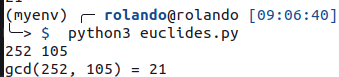
\includegraphics[width=10cm]{images/euclides_prueba.png}
        \caption{Ejecución de prueba del algoritmo de Euclides}
    \end{figure}

\subsection{ALGORITMO EXTENDIDO DE EUCLIDES}
El algoritmo extendido de Euclides, no solo encontrara los valores del Máximo Común Divisor (gcd) de dos números, sino también encontrara los valores de los coeficientes de Bézout, que son dos números tales que:
\[
    ax + by = gcd(a,b)
\]
    
    \subsubsection{IMPLEMENTACIÓN}
\begin{lstlisting}[language=Python]
def gcd_extendido(a, b):
if a == 0:
    return b, 0, 1
else:
    gcd, x1, y1 = gcd_extendido(b % a, a)
    x = y1 - (b // a) * x1
    y = x1
    return gcd, x, y
\end{lstlisting}
    
    \subsubsection{EJEMPLO NÚMERICO}
    Aplicamos el algoritmo de Euclides:
    \begin{align*} 
        252 &=  2\cdot105 + 42 \\ 
        105 &=  2\cdot42 + 21 \\
        42 &=  2\cdot21 + 0 \\ 
    \end{align*}
    
    Despejamos los residuos en los pasos del algoritmo de Euclides:

    \begin{align*} 
        42 &=  252 - 2\cdot105\\ 
        21 &=  105 - 2\cdot42\\ 
    \end{align*}

    Remplazamos 42 en la segunda ecuación:
    \begin{align*} 
        21 &=  105 - 2\cdot(252 - 2\cdot105)\\ 
        21 &=  105 - 2\cdot252 + 4\cdot105\\
        21 &=  2\cdot252 + 5\cdot105\\
        &\Rightarrow x = -2, y = 5 
    \end{align*}

    \subsubsection{EJEMPLO DE EJECUCIÓN}
    \begin{figure}[H]
        \centering
        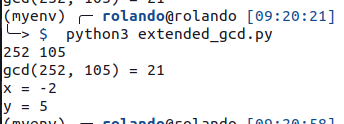
\includegraphics[width=10cm]{images/euclides_extendido_prueba.png}
        \caption{Ejecución de prueba del algoritmo extendido de Euclides}
    \end{figure}

\subsection{ALGORITMO DE EXPONENCIACIÓN MODULAR}
Con este algoritmo encontraremos de manera eficiente $f(x,a,m) = x^a \% m$
    \subsubsection{IMPLEMENTACIÓN}
\begin{lstlisting}[language=Python]
def mod_exp(base, exponente, modulo):
    resultado = 1
    base = base % modulo
    
    while exponente > 0:
        if (exponente % 2) == 1:
            resultado = (resultado * base) % modulo
        exponente = exponente >> 1
        base = (base * base) % modulo
    
    return resultado
\end{lstlisting}

    \subsubsection{EJEMPLO NÚMERICO}
    Encontrar el resultado para $25^9 \% 7$
    \begin{align*} 
        x &=  25^9 \% 7\\ 
        x &=  (25^4 \% 7)^2 (\times 25\cdot1) \% 7 \\
        x &=  ((25^2 \% 7)^2)^2 \times (25 \% 7)\\
        x &=  ((25\cdot25 \% 7)^2)^2 \times (25 \% 7)\\
        x &=  (((625 \% 7)^2)^2 \times 4)\%7\\
        x &=  (((2)^2)^2 \% 7 \times 4) mod 7\\
        x &= ((4^2)\% 7 \times 4) \% 7\\
        x &= (16 \% 7 \times 4) \% 7 \\
        x &= (2 \times 4) \% 7 \\
        x &= 8 \% 7 \\
        x &= 1
    \end{align*}

    \subsubsection{EJEMPLO DE EJECUCIÓN}
    \begin{figure}[H]
        \centering
        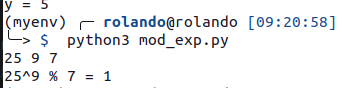
\includegraphics[width=10cm]{images/mod_exp_prueba.png}
        \caption{Ejecución de prueba del algoritmo de exponenciación modular}
    \end{figure}

\subsection{ALGORITMO DE DIVISIONES SUCESIVAS}
    \subsubsection{IMPLEMENTACIÓN}
\begin{lstlisting}[language=Python]
def divisiones_sucesivas(n):
    factores = []
    while n % 2 == 0:
        factores.append(2)
        n //= 2
    for i in range(3, int(n**0.5) + 1, 2):
        while n % i == 0:
            factores.append(i)
            n //= i
    if n > 2:
        factores.append(n)
    
    return factores
\end{lstlisting}

\subsubsection{EJEMPLO NÚMERICO}
Encontrar los factores primos de $1759875$, se prueba diviendo por todos los primos que sean $p_i$ tal que $p_i \leq \sqrt(n)$ y sean divisores de $n$.
\begin{align*} 
    1759875 / 3 & = 586625 \\
    586625 / 5 & = 117325 \\
    117325 / 5 & = 23465 \\
    23465 / 5 & =  4693\\
    4693 / 13 & =  361\\
    361 / 19 & =  19\\
    19 / 19 & =  1\\
    &\Rightarrow factores(1759875) = [3, 5^3, 13, 19^2]
\end{align*}

\subsubsection{EJEMPLO DE EJECUCIÓN}
\begin{figure}[H]
    \centering
    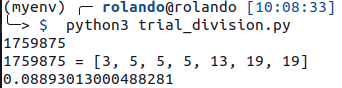
\includegraphics[width=10cm]{images/trial_divition_prueba.png}
    \caption{Ejecución de prueba del algoritmo de factorización por divisiones sucesivas}
\end{figure}


\subsection{MÉTODO DE DIFERENCIA DE CUADRADOS DE FERMAT}
\subsubsection{IMPLEMENTACIÓN}
\begin{lstlisting}[language=Python]
import math

def factorizacion_fermat(n):
    if n % 2 == 0:
        return (2, n // 2)

    a = math.ceil(math.sqrt(n))
    b2 = a * a - n

    while not es_cuadrado_perfecto(b2):
        a += 1
        b2 = a * a - n

    b = int(math.sqrt(b2))
    return (a - b, a + b)

def es_cuadrado_perfecto(x):
    s = int(math.isqrt(x))
    return s * s == x
\end{lstlisting}

\subsubsection{EJEMPLO NÚMERICO}
    Encontrar los factores primos de $5959$
    \begin{align*}
        a &= \lceil \sqrt{5959} \rceil \\
        a &= 78\\
        b^2 &= a^2 - n\\
        b^2 &= 78^2 - 5959\\
        b^2 &= 6084 - 5959\\
        b^2 &= 125
    \end{align*}
    Verificamos si $b^2$ es cuadrado perfecto:
    \begin{align*}
        \sqrt{125} & \approx 11.18 
    \end{align*}
    Como no es cuadrado perfecto se incrementa $a$ y se repite:
    \begin{align*}
        a &= 79\\
        b^2 &= 79^2 - 5959\\
        b^2 &= 282 \\
        \sqrt{282} &\approx 16.79 \\
        a &= 80\\
        b^2 &= 80^2 - 5959\\
        b^2 &= 441 \\
        \sqrt{441} &= 21 \\
    \end{align*}
    Como $441$ es cuadrado perfecto se han encontrado $a=80$ y $b=21$, y su factorización es:
    \begin{align*} 
        n &=  (a+b)(a-b)\\ 
        n &=  (80+21)(80-21)\\
        x &=  (101)(59)\\
    \end{align*}

    \subsubsection{EJEMPLO DE EJECUCIÓN}
    \begin{figure}[H]
        \centering
        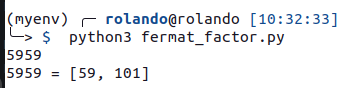
\includegraphics[width=10cm]{images/fermat_prueba.png}
        \caption{Ejecución de prueba del algoritmo de Fermat}
    \end{figure}

\subsection{ALGORITMO DE FACTORIZACIÓN EN UNA LINEA DE HART}
\subsubsection{IMPLEMENTACIÓN}
\begin{lstlisting}[language=Python]
import math

def factorizacion_hart(n, l):
    s = 1
    t = 1
    for i in range(1, l):
        s = math.ceil(math.sqrt(n*i))
        m = mod_exp(s, 2, n)
        t = math.isqrt(m)
        if t*t == m:
            break
    return gcd(s-t, n)
\end{lstlisting}
\subsubsection{EJEMPLO NÚMERICO}
    Factorizar $13290059$ con el algoritmo de factorización en una linea de Hart
    \begin{align*} 
        s &=  \lceil \sqrt{13290059\cdot 1}\rceil\\ 
        s &= 3646\\ 
        m &= 3646^2 \% 13290059\\ 
        m &= 3257\\
        \sqrt{m} &\approx  57.07\\
        \dots \\
        s &=  \lceil \sqrt{13290059\cdot 165}\rceil\\ 
        s &= 46828\\ 
        m &= 46828^2 \% 13290059\\
        m &= 1849\\
        t &=  \sqrt{m}\\
        t &=  \sqrt{1849}\\
        t &= 43\\
        gcd(s-t, n) &= gcd(46828-43, 13290059)\\
        &= 3119\\
    \end{align*}

    \subsubsection{EJEMPLO DE EJECUCIÓN}
    \begin{figure}[H]
        \centering
        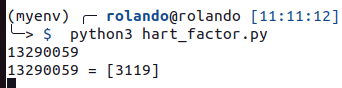
\includegraphics[width=10cm]{images/hart_prueba.png}
        \caption{Ejecución de prueba del algoritmo de factorización en una linea de Hart}
    \end{figure}


\subsection{MÉTODO DE POLLARD RHO}
\subsubsection{IMPLEMENTACIÓN}
\begin{lstlisting}[language=Python]
def pollard_rho(n):
    if n % 2 == 0:
        return 2

    x = random.randint(2, n - 1)
    y = x
    c = random.randint(1, n - 1)
    d = 1

    while d == 1:
        x = (mod_exp(x, 2, n) + c + n) % n
        y = (mod_exp(y, 2, n) + c + n) % n
        y = (mod_exp(y, 2, n) + c + n) % n
        d = gcd(abs(x - y), n)

    if d == n:
        return pollard_rho(n)

    return d
\end{lstlisting}

\subsubsection{EJEMPLO NÚMERICO}
    Factorizar $8051$ usando el algoritmo Pollard-Rho
    \begin{align*} 
        x &=  2\\
        y &=  2\\
        c &=  1\\ 
        d &= 1 \\
        x &= ((x^2)\%n + c + n)\%n\\
        x_0 &= (2^2\%8051 + 1 + 8051) \% 8051\\
        x_0 &= 5\\
        y_0 &= (2^2\%8051 + 1 + 8051) \% 8051\\
        y_0 &= 5\\
        y_1 &= (5^2\%8051 + 1 + 8051) \% 8051\\
        y_1 &= 26\\
        d &= gcd(|x-y|, n)\\
        d &= gcd(|5-26|, 8051)\\
        d &= 1
    \end{align*}

    \begin{align*} 
        x_1 &= (5^2\%8051 + 1 + 8051) \% 8051\\
        x_1 &= 26\\
        y_2 &= (26^2\%8051 + 1 + 8051) \% 8051\\
        y_2 &= 677\\
        y_3 &= (677^2\%8051 + 1 + 8051) \% 8051\\
        y_3 &= 7474\\
        d &= gcd(|26-7474|, 8051)\\
        d &= 1
    \end{align*}

    \begin{align*} 
        x_2 &= (26^2\%8051 + 1 + 8051) \% 8051\\
        x_2 &= 677\\
        y_2 &= (7474^2\%8051 + 1 + 8051) \% 8051\\
        y_2 &= 2839\\
        y_3 &= (2839^2\%8051 + 1 + 8051) \% 8051\\
        y_3 &= 871\\
        d &= gcd(|677-871|, 8051)\\
        d &= 97
    \end{align*}

    \subsubsection{EJEMPLO DE EJECUCIÓN}
    \begin{figure}[H]
        \centering
        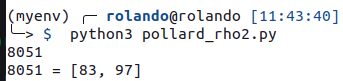
\includegraphics[width=10cm]{images/pollard_rho_prueba.png}
        \caption{Ejecución de prueba del algoritmo Pollard-Rho}
    \end{figure}

% \subsection{MÉTODO P-1 DE POLLARD}
% \subsubsection{IMPLEMENTACIÓN}
% \begin{lstlisting}[language=Python]
% import math
% from math import gcd
% from sympy import primerange

% def pollards_p_minus_1(n, B):
%     a = 2
    
%     M = 1
%     for p in primerange(2, B + 1)::
%         e = math.floor(math.log(n) / math.log(p))
%         M *= pow(p, e)
    
%     aM = mod_exp(a, M, n)
    
%     d = gcd(aM - 1, n)
    
%     if 1 < d < n:
%         return d
%     else:
%         return None
% \end{lstlisting}

% \subsubsection{EJEMPLO NÚMERICO}
%     Encontrar el resultado para $25^9 \% 7$
%     \begin{align*} 
%         x &=  25^9 \% 7\\ 
%         x &=  (25^4 \% 7)^2 (\times 25\cdot1) \% 7 \\
%         x &=  ((25^2 \% 7)^2)^2 \times (25 \% 7)\\
%         x &=  ((25\cdot25 \% 7)^2)^2 \times (25 \% 7)\\
%         x &=  (((625 \% 7)^2)^2 \times 4)\%7\\
%         x &=  (((2)^2)^2 \% 7 \times 4) mod 7\\
%         x &= ((4^2)\% 7 \times 4) \% 7\\
%         x &= (16 \% 7 \times 4) \% 7 \\
%         x &= (2 \times 4) \% 7 \\
%         x &= 8 \% 7 \\
%         x &= 1
%     \end{align*}

%     \subsubsection{EJEMPLO DE EJECUCIÓN}
%     \begin{figure}[H]
%         \centering
%         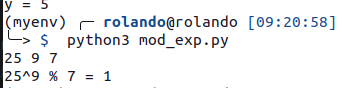
\includegraphics[width=10cm]{images/mod_exp_prueba.png}
%         \caption{Ejecución de prueba del algoritmo de exponenciación modular}
%     \end{figure}

\subsection{ALGORITMO DE FACTORIZACIÓN DE ENTEROS DE FRACCIONES CONTINUAS}
\subsubsection{IMPLEMENTACIÓN}
\begin{lstlisting}[language=Python]
import math

def fraccion_continua_sqrt(n):
    a0 = int(math.isqrt(n))
    if a0 * a0 == n:
        return [a0]
    
    cf = []
    m = 0
    d = 1
    a = a0
    cf.append(a)
    
    while a != 2 * a0:
        m = d * a - m
        d = (n - m * m) // d
        a = (a0 + m) // d
        cf.append(a)
    return cf

def convergentes(cf):
    h1, h2 = 1, 0
    k1, k2 = 0, 1
    convergentes_list = []
    
    for i in range(len(cf)):
        h = cf[i] * h1 + h2
        k = cf[i] * k1 + k2
        convergentes_list.append((h, k))
        h2, h1 = h1, h
        k2, k1 = k1, k
    return convergentes_list

def factorizar_fracciones_continuas(n):
    cf = fraccion_continua_sqrt(n)
    convs = convergentes(cf)
    
    for h, k in convs:
        if k == 0:
            continue
        x = h
        y = (x * x - n) // k
        
        if y >= 0 and int(math.isqrt(y)) ** 2 == y:
            factor = gcd(x + int(math.isqrt(y)), n)
            if 1 < factor < n:
                return factor
    
    return None
\end{lstlisting}

% \subsubsection{EJEMPLO NÚMERICO}
%     Encontrar el resultado para $25^9 \% 7$
%     \begin{align*} 
%         x &=  25^9 \% 7\\ 
%         x &=  (25^4 \% 7)^2 (\times 25\cdot1) \% 7 \\
%         x &=  ((25^2 \% 7)^2)^2 \times (25 \% 7)\\
%         x &=  ((25\cdot25 \% 7)^2)^2 \times (25 \% 7)\\
%         x &=  (((625 \% 7)^2)^2 \times 4)\%7\\
%         x &=  (((2)^2)^2 \% 7 \times 4) mod 7\\
%         x &= ((4^2)\% 7 \times 4) \% 7\\
%         x &= (16 \% 7 \times 4) \% 7 \\
%         x &= (2 \times 4) \% 7 \\
%         x &= 8 \% 7 \\
%         x &= 1
%     \end{align*}

    \subsubsection{EJEMPLO DE EJECUCIÓN}
    \begin{figure}[H]
        \centering
        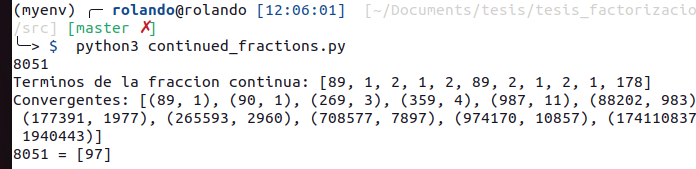
\includegraphics[width=10cm]{images/fracciones_continuas_pruebas.png}
        \caption{Ejecución de prueba del algoritmo de factorización con fracciones continuas}
    \end{figure}

\subsection{ALGORITMO DE FACTORIZACIÓN CON CURVAS ELÍPTICAS}
\subsubsection{IMPLEMENTACIÓN}
\begin{lstlisting}[language=Python]
def inverso_modular(a, p):
    g, x, _ = gcd_extendido(a, p)
    return x % p

def adicion_curva_eliptica(P, Q, a, p):
    if P == Q:
        lam = (3 * P[0] * P[0] + a) * inverso_modular(2 * P[1], p) % p
    else:
        lam = (Q[1] - P[1]) * inverso_modular(Q[0] - P[0], p) % p

    x3 = (lam * lam - P[0] - Q[0]) % p
    y3 = (lam * (P[0] - x3) - P[1]) % p

    return (x3, y3)

def multiplicacion_curva_eliptica(k, P, a, p):
    R = (0, 0)
    Q = P
    while k > 0:
        if k % 2 == 1:
            R = adicion_curva_eliptica(R, Q, a, p)
        Q = adicion_curva_eliptica(Q, Q, a, p)
        k //= 2
    return R

def ecm(n, B1=10000, B2=100000):
    while True:
        x = random.randint(1, n - 1)
        y = random.randint(1, n - 1)
        a = random.randint(1, n - 1)
        b = (y * y - x * x * x - a * x) % n

        if (4 * a * a * a + 27 * b * b) % n == 0:
            continue

        P = (x, y)
        for k in range(2, B1):
            P = multiplicacion_curva_eliptica(k, P, a, n)
            g = gcd(P[1], n)
            if 1 < g < n:
                return g


        for k in range(B1, B2):
            P = multiplicacion_curva_eliptica(k, P, a, n)
            g = gcd(P[1], n)
            if 1 < g < n:
                return g
\end{lstlisting}

% \subsubsection{EJEMPLO NÚMERICO}
%     Encontrar el resultado para $25^9 \% 7$
%     \begin{align*} 
%         x &=  25^9 \% 7\\ 
%         x &=  (25^4 \% 7)^2 (\times 25\cdot1) \% 7 \\
%         x &=  ((25^2 \% 7)^2)^2 \times (25 \% 7)\\
%         x &=  ((25\cdot25 \% 7)^2)^2 \times (25 \% 7)\\
%         x &=  (((625 \% 7)^2)^2 \times 4)\%7\\
%         x &=  (((2)^2)^2 \% 7 \times 4) mod 7\\
%         x &= ((4^2)\% 7 \times 4) \% 7\\
%         x &= (16 \% 7 \times 4) \% 7 \\
%         x &= (2 \times 4) \% 7 \\
%         x &= 8 \% 7 \\
%         x &= 1
%     \end{align*}

    \subsubsection{EJEMPLO DE EJECUCIÓN}
    \begin{figure}[H]
        \centering
        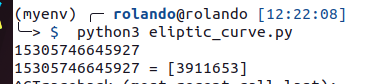
\includegraphics[width=10cm]{images/curva_eliptica_prueba.png}
        \caption{Ejecución de prueba del algoritmo de factorización con curvas Elipticas (ECM)}
    \end{figure}

\subsection{CRIBA DE ERATOSTENES}
\subsubsection{IMPLEMENTACIÓN}
\begin{lstlisting}[language=Python]
def sieve_of_eratosthenes(n):
    primes = [True] * (n + 1)
    p = 2
    while p * p <= n:
        if primes[p]:
            for i in range(p * p, n + 1, p):
                primes[i] = False
        p += 1
    return [p for p in range(2, n + 1) if primes[p]]
\end{lstlisting}
\subsubsection{EJEMPLO NÚMERICO}
    En la Figura \ref{eratostenes} se puede ver el resultado despues de ejecutar la criba de Eratostenes hasta 120, y a la derecha los primos encontrados
    \begin{figure}[H]
        \centering
        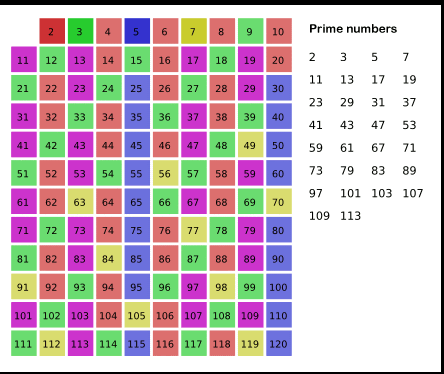
\includegraphics[width=10cm]{images/eratostenes_ejemplo.png}
        \caption{Resultado de la criba de Eratostenes}
        \label{eratostenes}
    \end{figure}

    % \subsubsection{EJEMPLO DE EJECUCIÓN}
    % \begin{figure}[H]
    %     \centering
    %     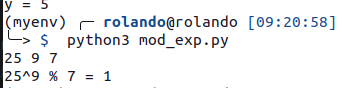
\includegraphics[width=10cm]{images/mod_exp_prueba.png}
    %     \caption{Ejecución de prueba del algoritmo de exponenciación modular}
    % \end{figure}

% \subsection{CRIBA MODIFICADA DE ERATOSTENES}
% \subsubsection{IMPLEMENTACIÓN}
% \begin{lstlisting}[language=Python]
% def sieve_interval_excluding_factors(I, J, P):
%     interval_size = J - I + 1
%     sieve = [True] * interval_size

%     for prime in P:
%         start = max(prime * prime, I + (prime - I % prime) % prime)
%         for multiple in range(start, J + 1, prime):
%             sieve[multiple - I] = False

    
%     result = [num for num, is_prime in zip(range(I, J + 1), sieve) if is_prime]
%     return result
% \end{lstlisting}

% \subsubsection{EJEMPLO NÚMERICO}
%     Encontrar el resultado para $25^9 \% 7$
%     \begin{align*} 
%         x &=  25^9 \% 7\\ 
%         x &=  (25^4 \% 7)^2 (\times 25\cdot1) \% 7 \\
%         x &=  ((25^2 \% 7)^2)^2 \times (25 \% 7)\\
%         x &=  ((25\cdot25 \% 7)^2)^2 \times (25 \% 7)\\
%         x &=  (((625 \% 7)^2)^2 \times 4)\%7\\
%         x &=  (((2)^2)^2 \% 7 \times 4) mod 7\\
%         x &= ((4^2)\% 7 \times 4) \% 7\\
%         x &= (16 \% 7 \times 4) \% 7 \\
%         x &= (2 \times 4) \% 7 \\
%         x &= 8 \% 7 \\
%         x &= 1
%     \end{align*}

%     \subsubsection{EJEMPLO DE EJECUCIÓN}
%     \begin{figure}[H]
%         \centering
%         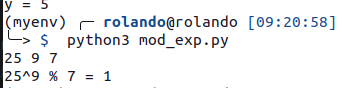
\includegraphics[width=10cm]{images/mod_exp_prueba.png}
%         \caption{Ejecución de prueba del algoritmo de exponenciación modular}
%     \end{figure}

\subsection{CRIBA CUADRATICA}
\subsubsection{IMPLEMENTACIÓN}
\begin{lstlisting}[language=Python]
def quad_residue(a,n):
    l=1
    q=(n-1)//2
    x = q**l
    if x==0:
        return 1
        
    a =a%n
    z=1
    while x!= 0:
        if x%2==0:
            a=(a **2) % n
            x//= 2
        else:
            x-=1
            z=(z*a) % n
    return z

def STonelli(n, p):
    q = p - 1
    s = 0
    while q % 2 == 0:
        q //= 2
        s += 1
    if s == 1:
        r = pow(n, (p + 1) // 4, p)
        return r,p-r
    for z in range(2, p):
        if p - 1 == quad_residue(z, p):
            break
    c = pow(z, q, p)
    r = pow(n, (q + 1) // 2, p)
    t = pow(n, q, p)
    m = s
    t2 = 0
    while (t - 1) % p != 0:
        t2 = (t * t) % p
        for i in range(1, m):
            if (t2 - 1) % p == 0:
                break
            t2 = (t2 * t2) % p
        b = pow(c, 1 << (m - i - 1), p)
        r = (r * b) % p
        c = (b * b) % p
        t = (t * c) % p
        m = i
    return (r,p-r)

def is_probable_prime(a):
    if a == 2:
        return True

    if a == 1 or a % 2 == 0:
        return False

    return rabin_miller_primality_test(a, 50)

def rabin_miller_primality_test(a, iterations):
    r, s = 0, a - 1

    while s % 2 == 0:
        r += 1
        s //= 2

    for _ in range(iterations):
        n = randint(2, a - 1)
        x = pow(n, s, a)
        if x == 1 or x == a - 1:
            continue
        for _ in range(r - 1):
            x = pow(x, 2, a)
            if x == a - 1:
                break
        else:
            return False
    return True

def prime_gen(n):
    if n < 2:
        return []
    
    nums = []
    isPrime = []
    
    for i in range(0, n+1):
        nums.append(i)
        isPrime.append(True)
        
    isPrime[0]=False
    isPrime[1]=False
    
    for j in range(2,int(n/2)):
        if isPrime[j] == True:
            for i in range(2*j,n+1,j):
                isPrime[i] = False
                
    primes = []
    for i in range(0, n+1):
        if isPrime[i] == True:
            primes.append(nums[i])
            
    return primes

def isqrt(n):
    x = n
    y = (x + 1) // 2
    while y < x:
        x = y
        y = (x + n // x) // 2
    return x

def find_base(N,B):
    factor_base = []
    primes = prime_gen(B)
    for p in primes:
        if quad_residue(N,p) == 1:
            factor_base.append(p)
    return factor_base

def find_smooth(factor_base,N,I):
    def sieve_prep(N,sieve_int):
        sieve_seq = [x**2 - N for x in range(root,root+sieve_int)]
        return sieve_seq

    sieve_seq = sieve_prep(N,I)
    sieve_list = sieve_seq.copy()
    if factor_base[0] == 2:
        i = 0
        while sieve_list[i] % 2 != 0:
            i += 1
        for j in range(i,len(sieve_list),2):
            while sieve_list[j] % 2 == 0:
                sieve_list[j] //= 2
    for p in factor_base[1:]:
        residues = STonelli(N,p)
        for r in residues:
            for i in range((r-root) % p, len(sieve_list), p):
                while sieve_list[i] % p == 0:
                    sieve_list[i] //= p
    xlist = []
    smooth_nums = []
    indices = []
    
    for i in range(len(sieve_list)):
        if len(smooth_nums) >= len(factor_base)+T:
            break
        if sieve_list[i] == 1:
            smooth_nums.append(sieve_seq[i])
            xlist.append(i+root)
            indices.append(i)
    return(smooth_nums,xlist,indices)

def build_matrix(smooth_nums,factor_base):
    def factor(n,factor_base):
        factors = []
        if n < 0:
            factors.append(-1)
        for p in factor_base:
            if p == -1:
                pass
            else:
                while n % p == 0:
                    factors.append(p)
                    n //= p
        return factors

    M = []
    factor_base.insert(0,-1)
    for n in smooth_nums:
        exp_vector = [0]*(len(factor_base))
        n_factors = factor(n,factor_base)
        for i in range(len(factor_base)):
            if factor_base[i] in n_factors:
                exp_vector[i] = (exp_vector[i] + n_factors.count(factor_base[i])) % 2
        if 1 not in exp_vector:
            return True, n
        else:
            pass
        
        M.append(exp_vector)
    return(False, transpose(M))

def transpose(matrix):
    new_matrix = []
    for i in range(len(matrix[0])):
        new_row = []
        for row in matrix:
            new_row.append(row[i])
        new_matrix.append(new_row)
    return(new_matrix)

def solve(solution_vec,smooth_nums,xlist,N):
    solution_nums = [smooth_nums[i] for i in solution_vec]
    x_nums = [xlist[i] for i in solution_vec]
    Asquare = 1
    for n in solution_nums:
        Asquare *= n
    b = 1
    for n in x_nums:
        b *= n
    a = isqrt(Asquare)
    factor = gcd(b-a,N)
    return factor

def solve_row(sol_rows,M,marks,K=0):
    solution_vec, indices = [],[]
    free_row = sol_rows[K][0]
    for i in range(len(free_row)):
        if free_row[i] == 1: 
            indices.append(i)
    for r in range(len(M)):
        for i in indices:
            if M[r][i] == 1 and marks[r]:
                solution_vec.append(r)
                break
            
    solution_vec.append(sol_rows[K][1])       
    return(solution_vec)

def gauss_elim(M):
    marks = [False]*len(M[0])
    
    for i in range(len(M)):
        row = M[i]
        for num in row:
            if num == 1:
                j = row.index(num)
                marks[j] = True
                
                for k in chain(range(0,i),range(i+1,len(M))):
                    if M[k][j] == 1:
                        for i in range(len(M[k])):
                            M[k][i] = (M[k][i] + row[i])%2
                break
    M = transpose(M)
    sol_rows = []
    for i in range(len(marks)):
        if marks[i]== False:
            free_row = [M[i],i]
            sol_rows.append(free_row)
    return sol_rows,marks,M

def QS(n,B,I):    
    global N
    global root
    global T
    N,root,K,T = n,int(sqrt(n)),0,1
    
    if isinstance(sqrt(N),int):
        return isqrt(N)
    factor_base = find_base(N,B)
    global F
    F = len(factor_base)
    smooth_nums,xlist,indices = find_smooth(factor_base, N,I)
    is_square, t_matrix = build_matrix(smooth_nums,factor_base)
    
    if is_square == True:
        x = smooth_nums.index(t_matrix)
        factor = gcd(xlist[x]+sqrt(t_matrix),N)
        return factor, N/factor
    sol_rows,marks,M = gauss_elim(t_matrix)
    solution_vec = solve_row(sol_rows,M,marks,0)
    factor = solve(solution_vec,smooth_nums,xlist,N)

    for K in range(1,len(sol_rows)):
        if (factor == 1 or factor == N):
            solution_vec = solve_row(sol_rows,M,marks,K)
            factor = solve(solution_vec,smooth_nums,xlist,N)
        else:
            return factor, int(N/factor)
\end{lstlisting}

\subsubsection{EJEMPLO DE EJECUCIÓN}
\begin{figure}[H]
    \centering
    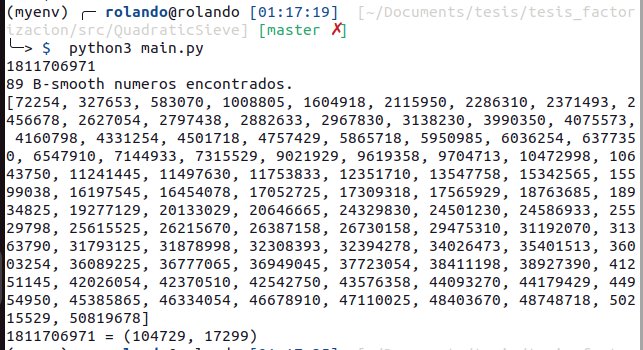
\includegraphics[width=10cm]{images/criba_cuadratica_prueba.png}
    \caption{Resultado de la criba de Cuadratica}
    \label{eratostenes}
\end{figure}
    \clearpage
\chapter{EVALUACIÓN DE RESULTADOS}
\section{GENERACIÓN DE CASOS DE PRUEBA}
Para la elaboración de los casos de prueba se utilizo el siguiente programa en python para lograr general los números compuestos con las características que necesitamos.
\begin{lstlisting}[language=Python]
def primos_aleatorios_menores_a(n):
    primos = list(map(int, primos_list))
    upper = binary_search(n, primos)
    for i in range(6, 23):
        number = 1
        fact = []
        while math.log10(number) < i:
            x = random.randint(0, upper)
            prime = primos[x]
            number = number * prime
            fact.append(prime)
        print(f'{number} = {fact}')


def binary_search(x, array):
    a = 0
    b = len(array)
    while(b-a > 1):
        c = math.floor((b+a)/2)
        if array[c] > x:
            b = c
        else:
            a = c
    return a


def dos_primos_mitad_digitos():
    primos = list(map(int, primos_list))
    for i in range(6, 18):
        lower = binary_search(pow(10, i/2), primos)
        upper = binary_search(pow(10, (i/2)+1), primos)
        n1 = random.randint(lower, upper+1)
        n2 = random.randint(lower, upper + 1)
        number = primos[n1] * primos[n2]
        fact = [primos[n1], primos[n2]]
        print(f'{number} = {fact}')


def dos_primos_cercanos():
    primos = list(map(int, primos_list))
    for i in range(6, 18):
        lower = binary_search(pow(10, i/2), primos)
        upper = binary_search(pow(10, (i/2)+1), primos)
        n1 = random.randint(lower, upper+1)
        n2 = n1 + random.randint(0, 100)*(-1**random.randint(0, 10))
        number = primos[n1] * primos[n2]
        fact = [primos[n1], primos[n2]]
        print(f'{number} = {fact}')
\end{lstlisting}

\section{RECOLECCIÓN DE DATOS}
Para evaluar las propiedades de los algoritmos de factorización de números enteros, se intentara factorizar diferentes números, de diferentes tamaños, y que cumplen ciertas propiedades, utilizando los algoritmos de Divisiones Sucesivas, Algoritmo de Fermat,Algoritmo de Pollard Rho, Método de factorización por curva elíptica y Criba Cuadrática, Se variaron los parámetros de entrada de cada algoritmo para evaluarlos en cuanto a tiempo de ejecución, memoria utilizada y factores primos encontrados.

Tenemos 3 conjuntos te números, en la Tabla \ref{tabla:factores_pequeños} tenemos el primer conjunto de números los cuales tienen la particularidad de tener varios factores primos pequeños.

\begin{table}[H]
    \begin{adjustbox}{width=\columnwidth,center}
    \centering
    \begin{tabular}{|c|c|c|}
    \hline
    Número a Factorizar & Cantidad de Dígitos & Factores Primos \\
    \hline
    10856663 & 8 & [2267, 4789] \\
33391459 & 8 & [4327, 7717] \\
52863301961 & 11 & [2903, 3257, 5591] \\
60176508803 & 11 & [2399, 4931, 5087] \\
198506677433 & 12 & [2459, 8839, 9133] \\
212154123015013 & 15 & [2909, 3221, 4057, 5581] \\
224446720764659 & 15 & [1019, 3571, 6269, 9839] \\
178466784060619 & 15 & [577, 3527, 8933, 9817] \\
191470730623531 & 15 & [1373, 2347, 6361, 9341] \\
1422516521828333 & 16 & [3797, 4391, 9001, 9479] \\
1151160785730511661 & 19 & [7, 479, 1069, 5653, 6367, 8923] \\
188790832382174409613 & 21 & [97, 1949, 2243, 6571, 7057, 9601] \\
1020515758802666029 & 19 & [607, 2663, 7621, 8861, 9349] \\
1724030839771633601827 & 22 & [431, 2333, 3359, 6709, 8369, 9091] \\
5433376091934805169983 & 22 & [599, 4001, 5393, 6067, 7927, 8741] \\
1524997222903385596412591 & 25 & [887, 1877, 2767, 2969, 3049, 3889, 9403] \\
39926046905882865492053 & 23 & [643, 821, 1213, 1613, 2143, 2797, 6449] \\
    \hline
    \end{tabular}
\end{adjustbox}
    \caption{Casos de prueba: factores pequeños}
    \label{tabla:factores_pequeños}
    

\end{table}
    

En la Tabla \ref{tabla:factores_mitad} tenemos el siguiente conjunto de casos de prueba los cuales son el producto de dos números primos de aproximadamente la mitad de dígitos.

\begin{table}[H]
    \centering
    \begin{tabular}{|c|c|c|}
    \hline
    Número a Factorizar & Cantidad de Dígitos & Factores Primos \\
    \hline
    16236991 & 8 & [3361, 4831] \\
    469526207 & 9 & [18587, 25261] \\
    914465141 & 9 & [20731, 44111] \\
    45774604399 & 11 & [211193, 216743] \\
    138426627499 & 12 & [225343, 614293] \\
    2002311773621 & 13 & [703709, 2845369] \\
    36162913278367 & 14 & [4352419, 8308693] \\
    279747589361921 & 15 & [9353483, 29908387] \\
    3064287451898711 & 16 & [38873827, 78826493] \\
    6587155271801233 & 16 & [64776983, 101689751] \\
    853877380996470053 & 18 & [893082227, 956101639] \\
    831279571604286949 & 18 & [849122999, 978986051] \\
    37351160168752886641 & 20 & [5814185473, 6424143217] \\
    \hline
    \end{tabular}
    \caption{Casos de prueba: Dos primos de la mitad de dígitos}
    \label{tabla:factores_mitad}
    \end{table}
    

En la Tabla \ref{tabla:primos_cercanos} se encuentra el ultimo conjunto de casos de prueba los cuales son producto de dos números primos cercanos.

\begin{table}[H]
    \centering
    \begin{tabular}{|c|c|c|}
    \hline
    Número a Factorizar & Cantidad de Dígitos & Factores Primos \\
    \hline
66436879 & 8 & [8017, 8287] \\
686703811 & 9 & [25981, 26431] \\
8101438039 & 10 & [89963, 90053] \\
85526931211 & 11 & [292183, 292717] \\
262209534767 & 12 & [511991, 512137] \\
715281207649 & 12 & [845623, 845863] \\
1873966393597 & 13 & [1368467, 1369391] \\
18701749916023 & 14 & [4324261, 4324843] \\
1757788889012333 & 16 & [41925839, 41926147] \\
34843998810184129 & 17 & [186665113, 186665833] \\
874655409151893869 & 18 & [935229067, 935231207] \\
286073409635796583 & 18 & [534857399, 534859217] \\
    \hline
    \end{tabular}
    \caption{Casos de prueba: Dos primos cercanos}
    \label{tabla:primos_cercanos}
    \end{table}
    

% Para cada uno de los algoritmos mencionados se presentara el mismo conjunto de números a factorizar, estos tendrán diferentes características y tamaños, podemos ver estos números en la Tabla 4.1.

% \begin{table}[H]
%     \centering
%     \begin{tabular}{ccc}
%     \toprule
%     Número a factorizar & Cantidad de Dígitos & Factores primos\\
%     \midrule
%     189031 & 6 & 19 * 9949\\
%     162167 & 6 & 257 * 631 \\
%     129859 & 6 & 31 * 59 * 71\\
%     1456489 & 7 & 157 * 9277\\
%     4051247 & 7 & 1607 * 2521\\
%     1759875 & 7 & 3 * 5*5*5*13*19*19 \\
%     12345679 & 8 & 37 * 900361\\
%     47934097 & 8 & 5101 * 9397\\
%     61247841 & 8 & 3 * 59 * 293 * 1181\\
%     13290059 & 8 & 3119 * 4261\\
%     299944727 & 9 & 15013 * 19979\\
%     123456797 & 9 & 73 * 1691189\\
%     106418569 & 9 & 7901*13469\\
%     182552955 & 9 & 3*5 * 13 * 13*23*31*101\\
%     9872747167 & 10 & 71*9871*14087\\
%     1040594999 & 10 & 25453 * 40883\\
%     98765432101 & 11 & 7* 149* 94693607\\
%     98765432057 & 11 & 41 * 2408912977\\
%     29111611559 & 11 & 69763*417293\\
%     947452370929 & 12 & 597827*1584827\\
%     254903331620 & 12 & 2*2*5*7*137*13290059\\
%     5228595324973 & 13 & 7501367*697019\\
%     47096679270259 & 14 & 3986929*11812771\\
%     235308795456937 & 15 & 13895201*16934537\\
%     1536588216289253 & 16 & 27801481*55270013\\
%     71453335284995017 & 17 & 155267159*460196063\\
%     57639038785408205 & 17 & 5*107367629*107367629\\
%     123456789012345678 & 18 & 2*3*3*3*21491747*106377431\\
%     542588624267342771 & 18 & 999997717*542589863\\
%     75557863725914323419137 & 23 & 17 · 1217 · 148961 · 24517014940753\\
%     \bottomrule
%     \end{tabular}
%     \caption{Conjunto de casos de prueba}
%     \label{tab:test-cases}
% \end{table}

% Los anteriores números fueron escogidos bajo algún criterio, como ser que varios son producto de dos números primos de la mitad de digitos que el número a factorizar o que tengan factores primos cercanos entre si. Adicionalmente se probara con un conjunto aleatorio de números, los cuales se muestran en la siguiente tabla.

% \begin{table}[h!]
%     \centering
%     \begin{tabular}{ccc}
%     \toprule
%     Número a factorizar & Cantidad de Dígitos & Factores primos\\
%     \midrule
%     4301669863 & 10 & 19 * 9949\\
%     4474219569 & 10 & 19 * 9949\\
%     4664207327 & 10 & 19 * 9949\\
%     3058913425 & 10 & 19 * 9949\\
%     8483408929 & 10 & 19 * 9949\\
%     91157961540 & 11 & 19 * 9949\\
%     71834755526 & 11 & 19 * 9949\\
%     19273835063 & 11 & 19 * 9949\\
%     94619342089 & 11 & 19 * 9949\\
%     35787761525 & 11 & 19 * 9949\\
%     666487305812 & 12 & 19 * 9949\\
%     33597589296 & 11 & 19 * 9949\\
%     998954783887 & 12 & 19 * 9949\\
%     347170454804 & 12 & 19 * 9949\\
%     973310845497 & 12 & 19 * 9949\\
%     326766468166 & 12 & 19 * 9949\\
%     7801713685685 & 13 & 19 * 9949\\
%     2668814811683 & 13 & 19 * 9949\\
%     5166123625339 & 13 & 19 * 9949\\
%     1496809063452 & 13 & 19 * 9949\\
%     2381216947725 & 13 & 19 * 9949\\
%     9644598203024 & 13 & 19 * 9949\\
%     10767704951543 & 14 & 19 * 9949\\
%     39668435387513 & 14 & 19 * 9949\\
%     68567173978082 & 14 & 19 * 9949\\
%     626274576394575 & 15 & 19 * 9949\\
%     737718941804106 & 15 & 19 * 9949\\
%     801604699212680 & 15 & 19 * 9949\\
%     452737951177671 & 15 & 19 * 9949\\
%     651530963341522 & 15 & 19 * 9949\\
%     9042898512612678 & 16 & 19 * 9949\\
%     6834126780084647 & 16 & 19 * 9949\\
%     1975605261582842 & 16 & 19 * 9949\\
%     4052906513611024 & 16 & 19 * 9949\\
%     4218681717928292 & 16 & 19 * 9949\\
%     65120691164835513 & 17 & 19 * 9949\\
%     81771695091271478 & 17 & 19 * 9949\\
%     40037231406989079 & 17 & 19 * 9949\\
%     73220842553719932 & 17 & 19 * 9949\\
%     71476068120491844 & 17 & 19 * 9949\\
%     \bottomrule
%     \end{tabular}
%     \caption{Resultados del Modelo de Erdős-Rényi}
%     \label{tab:erdos-renyi}
% \end{table}

\section{RESULTADOS}
    \subsection{DIVISIONES SUCESIVAS}
    El algoritmo de divisiones sucesivas tiene una complejidad temporal de $O(\sqrt{n})$ en el peor caso y una complejidad espacial de $O(1)$. Se espera que este algoritmo se comporte bien cuando los factores primos son pequeños y en cuanto el factor más grande crezca este algoritmo dejara de ser adecuado. 

    Primero se realizara las pruebas con los casos de prueba de la Tabla \ref{tabla:factores_pequeños}
    
    \begin{table}[H]
        \centering
        \begin{adjustbox}{width=\columnwidth,center}
        \begin{tabular}{ccc}
        \toprule
        Número a factorizar & Tiempo de ejecución (ms) & Factores primos encontrados\\
        \midrule
        10856663 & 0.310 & [2267, 4789]\\
        33391459 & 0.464 & [4327, 7717]\\
        52863301961 & 0.386 & [2903, 3257, 5591]\\
        60176508803 & 0.339 & [2399, 4931, 5087]\\
        198506677433 & 0.555 & [2459, 8839, 9133]\\
        212154123015013 & 0.354 & [2909, 3221, 4057, 5581]\\
        224446720764659 & 0.570 & [1019, 3571, 6269, 9839]\\
        178466784060619 & 0.554 & [577, 3527, 8933, 9817]\\
        191470730623531 & 0.585 & [1373, 2347, 6361, 9341]\\
        1422516521828333 & 0.580 & [3797, 4391, 9001, 9479]\\
        1151160785730511661 & 0.545 & [7, 479, 1069, 5653, 6367, 8923]\\
        188790832382174409613 & 0.629 & [97, 1949, 2243, 6571, 7057, 9601]\\
        1020515758802666029 & 0.618 & [607, 2663, 7621, 8861, 9349]\\
        1724030839771633601827 & 0.652 & [431, 2333, 3359, 6709, 8369, 9091]\\
        5433376091934805169983 & 0.565 & [599, 4001, 5393, 6067, 7927, 8741]\\
        1524997222903385596412591 & 0.627 & [887, 1877, 2767, 2969, 3049, 3889, 9403]\\
        39926046905882865492053 & 0.434 & [643, 821, 1213, 1613, 2143, 2797, 6449]\\

        \bottomrule
        \end{tabular}
        \end{adjustbox}
    \caption{Resultados del Algoritmo de Divisiones Sucesivas para el conjunto de casos de prueba de la Tabla \ref{tabla:factores_pequeños}}
        \label{tab:res-trial_1}
    \end{table}

   Y ahora se realizara las pruebas con los casos de prueba de la Tabla \ref{tabla:factores_mitad}

    \begin{table}[H]
        \centering
        \begin{tabular}{ccc}
        \toprule
        Número a factorizar & Tiempo de ejecución (ms) & Factores primos encontrados\\
        \midrule
        16236991 & 0.295 & [3361, 4831]\\
        469526207 & 1.523 & [18587, 25261]\\
        914465141 & 2.715 & [20731, 44111]\\
        45774604399 & 14.768 & [211193, 216743]\\
        138426627499 & 37.848 & [225343, 614293]\\
        2002311773621 & 183.913 & [703709, 2845369]\\
        36162913278367 & 582.346 & [4352419, 8308693]\\
        279747589361921 & 2058.641 & [9353483, 29908387]\\
        3064287451898711 & 5634.140 & [38873827, 78826493]\\
        6587155271801233 & 7452.034 & [64776983, 101689751]\\
        853877380996470053 & 80050.156 & [893082227, 956101639]\\
        831279571604286949 & 76501.414 & [849122999, 978986051]\\
        37351160168752886641 & 768585.739 & [5814185473, 6424143217]\\

        \bottomrule
        \end{tabular}
        \caption{Resultados del Algoritmo de Divisiones Sucesivas para el conjunto de casos de prueba de la Tabla \ref{tabla:factores_mitad}}
        \label{tab:res-trial_2}
    \end{table}

    \begin{table}[H]
        \centering
        \begin{tabular}{ccc}
        \toprule
        Número a factorizar & Tiempo de ejecución (ms) & Factores primos encontrados\\
        \midrule
        66436879 & 0.437 & [8017, 8287]\\
        686703811 & 1.394 & [25981, 26431]\\
        8101438039 & 6.293 & [89963, 90053]\\
        85526931211 & 21.026 & [292183, 292717]\\
        262209534767 & 39.504 & [511991, 512137]\\
        715281207649 & 64.788 & [845623, 845863]\\
        1873966393597 & 109.328 & [1368467, 1369391]\\
        18701749916023 & 339.266 & [4324261, 4324843]\\
        1757788889012333 & 3414.500 & [41925839, 41926147]\\
        34843998810184129 & 15096.030 & [186665113, 186665833]\\
        874655409151893869 & 81195.058 & [935229067, 935231207]\\
        286073409635796583 & 43553.943 & [534857399, 534859217]\\

        \bottomrule
        \end{tabular}
        \caption{Resultados del Algoritmo de Divisiones Sucesivas para el conjunto de casos de prueba de la Tabla \ref{tabla:primos_cercanos}}
        \label{tab:res-trial-cercanos}
    \end{table}

    Como se puede ver este algoritmo funciona bastante bien cuando se tiene factores primos pequeños pero el tiempo de ejecución crece en gran medida cuando se tienen factores primos muy grandes y también se puede ver que este algoritmo devuelve todos los factores primos de los números a factorizar. Esto se puede notar mejor en el gráfico de la Figura \ref{fig:res-trial}
    

    \begin{figure}[H]
        \centering
        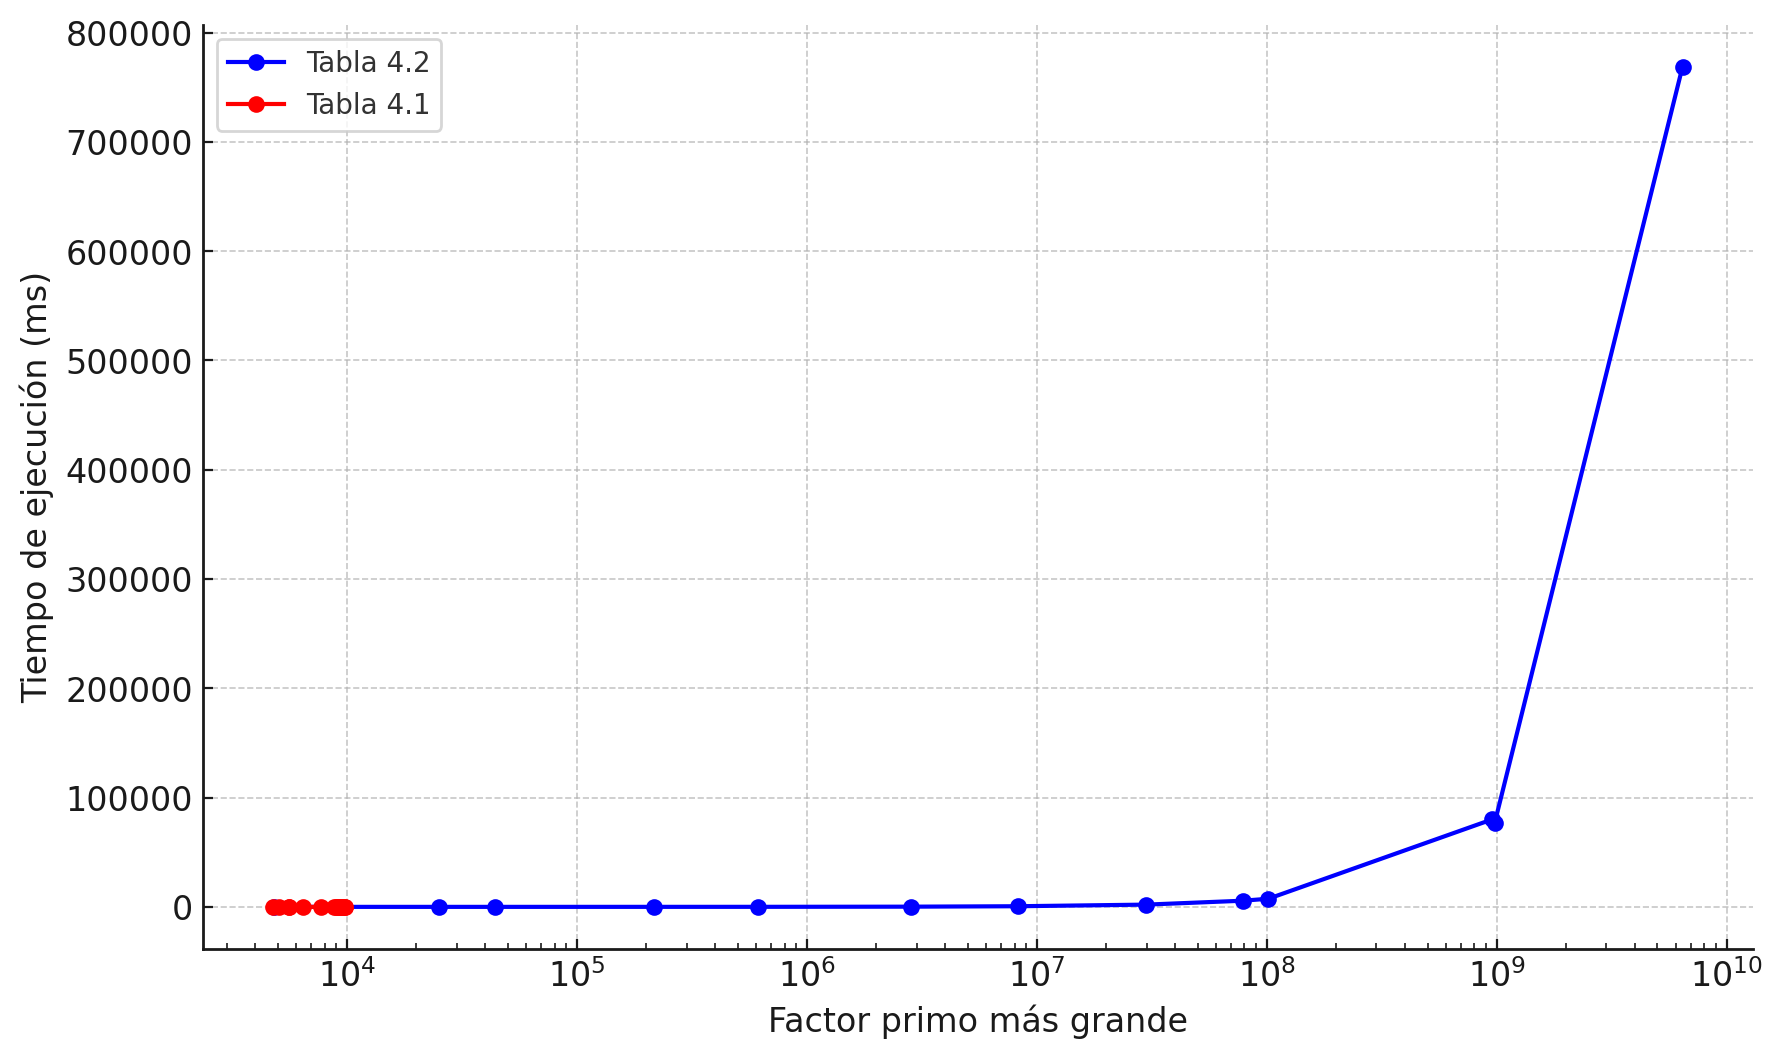
\includegraphics[width=\linewidth]{images/trial_divition3.png}
        \caption{Resultados Algoritmo de Divisiones Sucesivas}
        \label{fig:res-trial}
    \end{figure}

    \subsection{MÉTODO DE DIFERENCIA DE CUADRADOS DE FERMAT}
    El método de diferencia de cuadrados de Fermat tiene una complejidad temporal de $O(\sqrt{n})$ en el peor caso y una complejidad espacial de $O(1)$. Se espera que este algoritmo se desenvuelva bien cuando los factores primos sean cercanos y por la naturaleza de este algoritmo solo devolverá dos factores como resultado.

    Por este motivo primero se ejecutara el algoritmo con los casos de prueba de la Tabla \ref{tabla:factores_mitad}

    \begin{table}[H]
        \centering
        \begin{tabular}{ccc}
        \toprule
        Número a factorizar & Tiempo de ejecución (ms) & Factores primos encontrados\\
        \midrule
        16236991 & 0.026 & (3361, 4831)\\
        469526207 & 0.091 & (18587, 25261)\\
        914465141 & 0.602 & (20731, 44111)\\
        45774604399 & 0.007 & (211193, 216743)\\
        138426627499 & 13.287 & (225343, 614293)\\
        2002311773621 & 101.312 & (703709, 2845369)\\
        36162913278367 & 91.956 & (4352419, 8308693)\\
        279747589361921 & 879.645 & (9353483, 29908387)\\
        3064287451898711 & 1034.177 & (38873827, 78826493)\\
        6587155271801233 & 614.972 & (64776983, 101689751)\\
        853877380996470053 & 159.865 & (893082227, 956101639)\\
        831279571604286949 & 688.792 & (849122999, 978986051)\\
        37351160168752886641 & 2511.930 & (5814185473, 6424143217)\\
        \bottomrule
        \end{tabular}
        \caption{Resultados del Método de diferencia de cuadrados de Fermat con casos de prueba de la Tabla \ref{tabla:factores_mitad}}
        \label{tab:res-fermat-mitad}
    \end{table}

    Ahora se ejecutara el algoritmo con los casos de prueba de la Tabla \ref{tabla:primos_cercanos}, y se observara los resultados obtenidos:

    \begin{table}[H]
        \centering
        \begin{tabular}{ccc}
        \toprule
        Número a factorizar & Tiempo de ejecución (ms) & Factores primos encontrados\\
        \midrule
        66436879 & 0.009 & (8017, 8287)\\
        686703811 & 0.030 & (25981, 26431)\\
        8101438039 & 0.036 & (89963, 90053)\\
        85526931211 & 0.003 & (292183, 292717)\\
        262209534767 & 0.002 & (511991, 512137)\\
        715281207649 & 0.002 & (845623, 845863)\\
        1873966393597 & 0.002 & (1368467, 1369391)\\
        18701749916023 & 0.002 & (4324261, 4324843)\\
        1757788889012333 & 0.002 & (41925839, 41926147)\\
        34843998810184129 & 0.002 & (186665113, 186665833)\\
        874655409151893869 & 0.002 & (935229067, 935231207)\\
        286073409635796583 & 0.002 & (534857399, 534859217)\\
        \bottomrule
        \end{tabular}
        \caption{Resultados del Método de diferencia de cuadrados de Fermat con casos de prueba de la Tabla \ref{tabla:primos_cercanos}}
        \label{tab:res-fermat-cercano}
    \end{table}

    Se puede ver que este algoritmo funciona mejor cuando la distancia entre ambos factores es pequeña, lo cual puede ser visto de manera gráfica en la Figura \ref{fig:res-fermat}

    \begin{figure}[H]
        \centering
        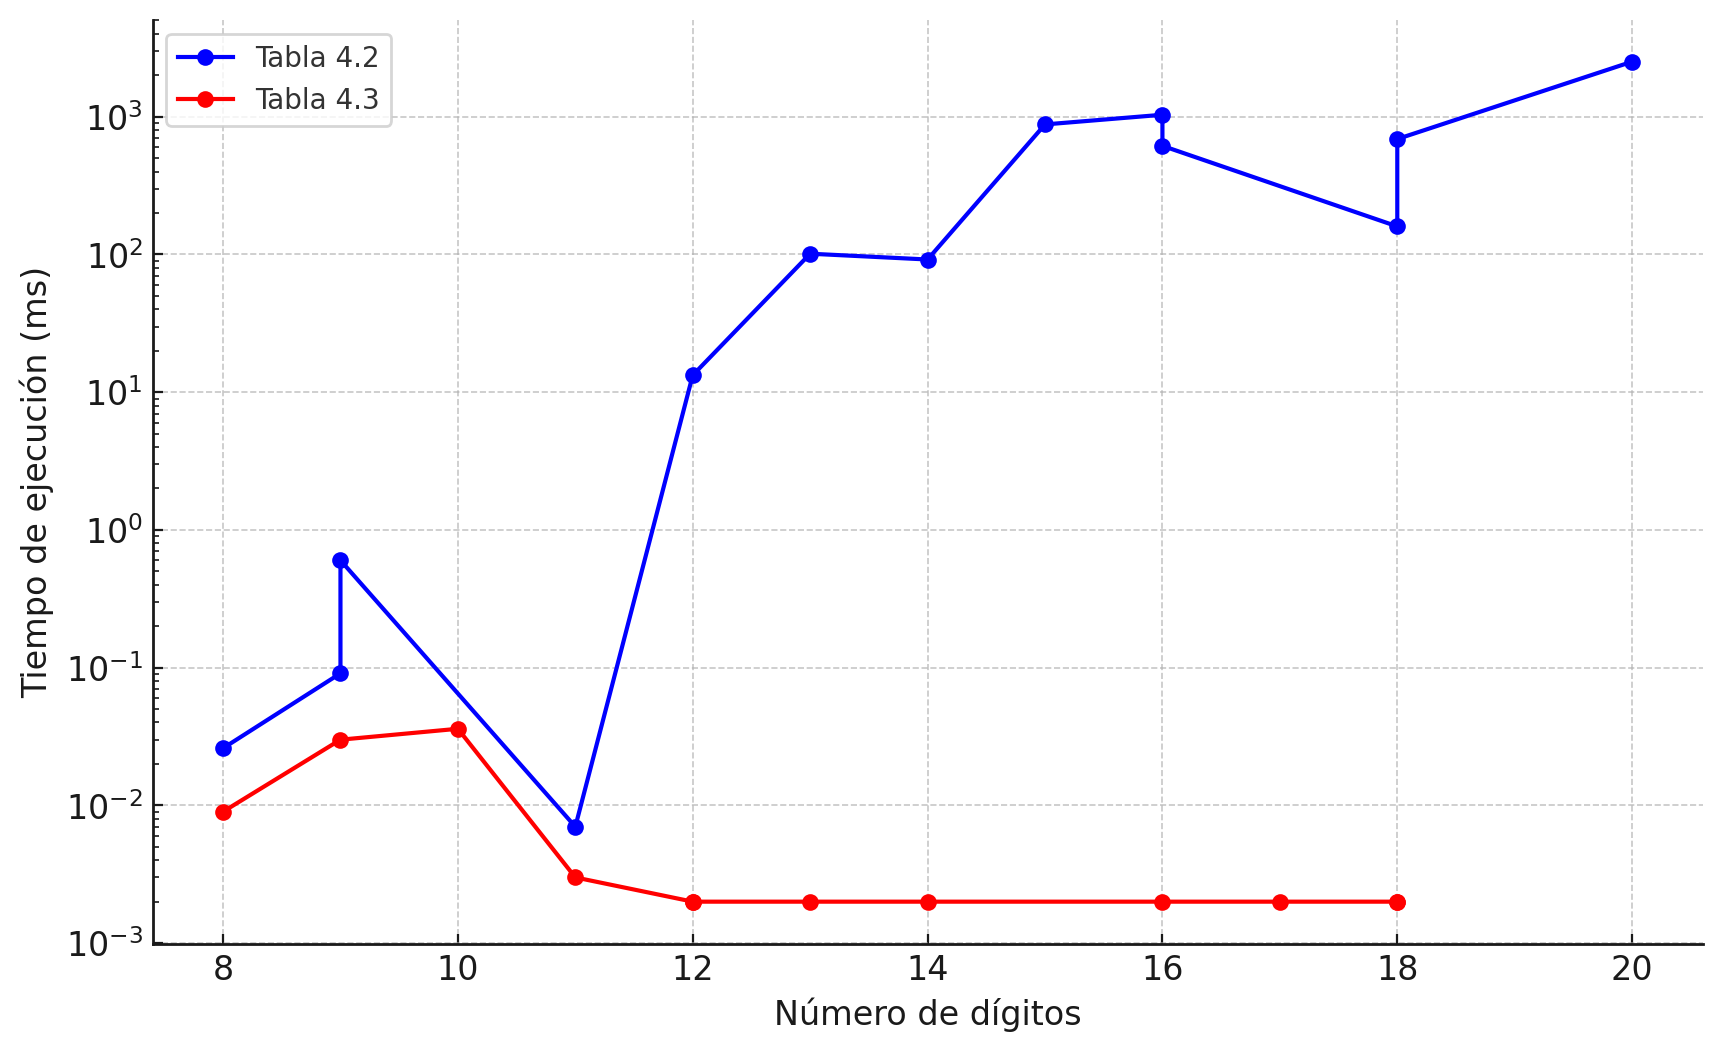
\includegraphics[width=\linewidth]{images/fermat_result.png}
        \caption{Resultados Método de diferencia de cuadrados de Fermat}
        \label{fig:res-fermat}
    \end{figure}

    \subsection{ALGORITMO DE POLLARD RHO}
    El algoritmo de Pollard Rho tiene una complejidad temporal de $O(n^{1/4})$ en el peor caso y una complejidad espacial de $O(1)$. Se espera que este algoritmo de uso general funcione bien para multiples casos.

    Comenzamos con los casos de prueba de la Tabla \ref{tabla:factores_pequeños}, que son números que tienen factores primos pequeños.

    \begin{table}[H]
        \centering
        \begin{adjustbox}{width=\columnwidth,center}
        \begin{tabular}{ccc}
        \toprule
        Número a factorizar & Tiempo de ejecución (ms) & Factores primos encontrados\\
        \midrule
        10856663 & 0.124 & [2267, 4789]\\
        33391459 & 0.035 & [4327, 7717]\\
        52863301961 & 0.219 & [2903, 3257, 5591]\\
        60176508803 & 0.181 & [2399, 4931, 5087]\\
        198506677433 & 0.242 & [2459, 9133, 8839]\\
        212154123015013 & 0.206 & [2909, 4057, 5581, 3221]\\
        224446720764659 & 0.324 & [1019, 9839, 3571, 6269]\\
        178466784060619 & 0.175 & [9817, 8933, 577, 3527]\\
        191470730623531 & 0.455 & [9341, 1373, 2347, 6361]\\
        1422516521828333 & 0.316 & [9479, 3797, 4391, 9001]\\
        1151160785730511661 & 0.656 & [7, 479, 1069, 8923, 5653, 6367]\\
        188790832382174409613 & 0.484 & [97, 7057, 6571, 1949, 2243, 9601]\\
        1020515758802666029 & 0.442 & [607, 7621, 2663, 8861, 9349]\\
        1724030839771633601827 & 0.481 & [431, 2333, 3359, 9091, 8369, 6709]\\
        5433376091934805169983 & 0.494 & [599, 4001, 8741, 7927, 5393, 6067]\\
        1524997222903385596412591 & 0.506 & [887, 2969, 3889, 1877, 2767, 3049, 9403]\\
        39926046905882865492053 & 0.316 & [1613, 995873, 643, 5993971, 6449]\\
        \bottomrule
        \end{tabular}
        \end{adjustbox}

        \caption{Resultados del Método de Pollard Rho con casos de la Tabla \ref{tabla:factores_pequeños}}
        \label{tab:res-pollard-rho-pequeños}
    \end{table}

    Ahora usaremos los casos de prueba de la Tabla \ref{tabla:factores_mitad}:

    \begin{table}[H]
        \centering
        \begin{tabular}{ccc}
        \toprule
        Número a factorizar & Tiempo de ejecución (ms) & Factores primos encontrados\\
        \midrule
        16236991 & 0.103 & [3361, 4831]\\
        469526207 & 0.215 & [25261, 18587]\\
        914465141 & 0.357 & [20731, 44111]\\
        45774604399 & 1.069 & [211193, 216743]\\
        138426627499 & 1.070 & [225343, 614293]\\
        2002311773621 & 1.553 & [703709, 2845369]\\
        36162913278367 & 4.246 & [4352419, 8308693]\\
        279747589361921 & 2.086 & [9353483, 29908387]\\
        3064287451898711 & 7.950 & [38873827, 78826493]\\
        6587155271801233 & 21.058 & [101689751, 64776983]\\
        853877380996470053 & 87.079 & [893082227, 956101639]\\
        831279571604286949 & 60.720 & [978986051, 849122999]\\
        37351160168752886641 & 64.655 & [6424143217, 5814185473]\\
        \bottomrule
        \end{tabular}
        \caption{Resultados del Método de Pollard Rho con casos de la Tabla \ref{tabla:factores_mitad}}
        \label{tab:res-pollard-rho-mitad}
    \end{table}

    Y por ultimo ejecutaremos el algoritmo con los casos de prueba de la Tabla \ref{tabla:primos_cercanos}
    
    \begin{table}[H]
        \centering
        \begin{tabular}{ccc}
        \toprule
        Número a factorizar & Tiempo de ejecución (ms) & Factores primos encontrados\\
        \midrule
        66436879 & 0.213 & [8287, 8017]\\
        686703811 & 0.235 & [25981, 26431]\\
        8101438039 & 0.280 & [90053, 89963]\\
        85526931211 & 2.490 & [292717, 292183]\\
        262209534767 & 1.729 & [511991, 512137]\\
        715281207649 & 1.384 & [845623, 845863]\\
        1873966393597 & 1.494 & [1369391, 1368467]\\
        18701749916023 & 0.481 & [4324843, 4324261]\\
        1757788889012333 & 15.424 & [41926147, 41925839]\\
        34843998810184129 & 14.593 & [186665113, 186665833]\\
        874655409151893869 & 62.654 & [935231207, 935229067]\\
        286073409635796583 & 11.130 & [534857399, 534859217]\\
        \bottomrule
        \end{tabular}
        \caption{Resultados del Método de Pollard Rho con casos de la Tabla \ref{tabla:primos_cercanos}}
        \label{tab:res-pollard-rho-cercanos}
    \end{table}

    En general para cualquier número Pollard-Rho tiene un tiempo de ejecución aceptable, con tiempos que no exceden los $100ms$ para nuestros casos de prueba, como se puede ver en la Figura \ref{fig:res-pollard-rho}.

    \begin{figure}[H]
        \centering
        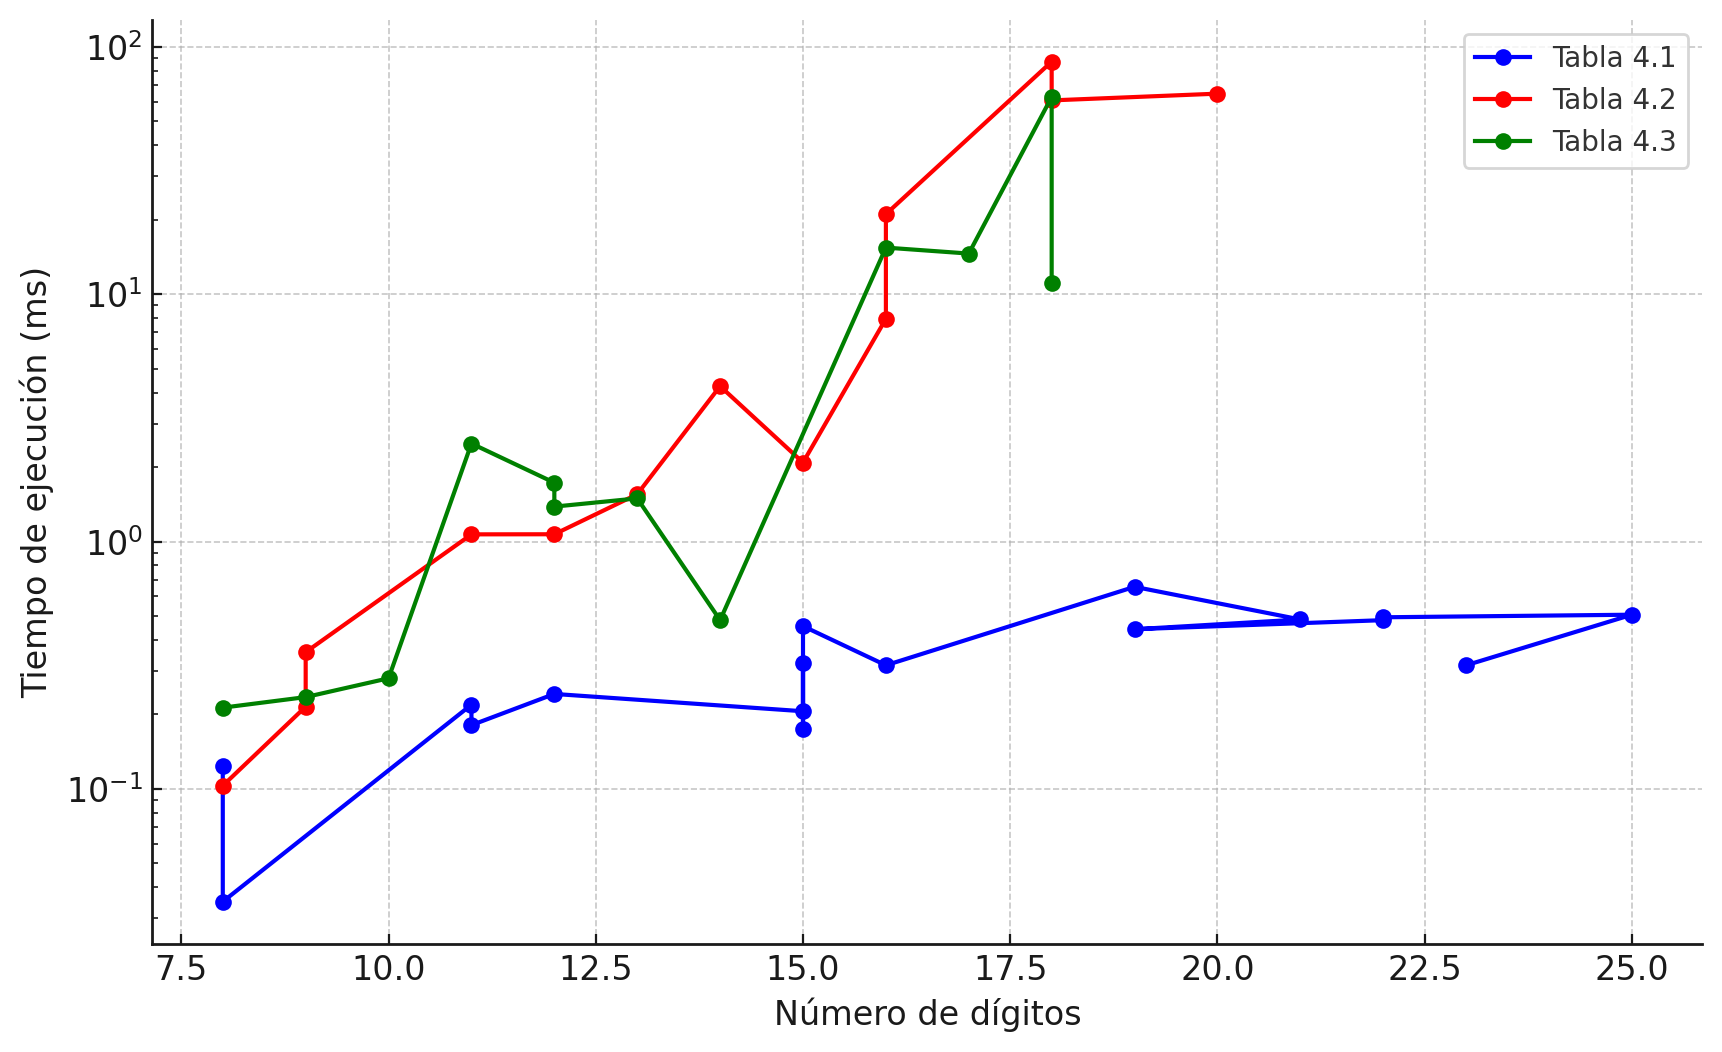
\includegraphics[width=\linewidth]{images/res-pollard-rho.png}
        \caption{Resultados Algoritmo de Pollard Rho}
        \label{fig:res-pollard-rho}
    \end{figure}

    \subsection{MÉTODO DE FACTORIZACIÓN CON CURVAS ELIPTICAS}
    El método de factorización con Curvas Elipticas tiene una complejidad temporal de \\ $O(e^{\sqrt{2 \log p \log \log p}})$ en el peor caso y una complejidad espacial de $O(\log n)$.

    \begin{table}[H]
        \centering
        \begin{tabular}{ccc}
        \toprule
        Número a factorizar & Tiempo de ejecución (ms) & Factores primos encontrados\\
        \midrule
        10856663 & 8.789 & 2267\\
        33391459 & 41.456 & 4327\\
        52863301961 & 15.100 & 2903\\
        60176508803 & 134.888 & 2399\\
        198506677433 & 274.809 & 2459\\
        212154123015013 & 28.153 & 2909\\
        224446720764659 & 224.039 & 1019\\
        178466784060619 & 2.281 & 577\\
        191470730623531 & 61.980 & 1373\\
        1422516521828333 & 67.354 & 4391\\
        1151160785730511661 & 0.041 & 7\\
        188790832382174409613 & 18.549 & 97\\
        1020515758802666029 & 1.148 & 607\\
        1724030839771633601827 & 9.571 & 3359\\
        5433376091934805169983 & 9.329 & 599\\
        1524997222903385596412591 & 22.790 & 2969\\
        39926046905882865492053 & 17.009 & 643\\

        \bottomrule
        \end{tabular}
        \caption{Resultados del Método de Factorización con Curvas Elipticas para los casos de prueba de la Tabla \ref{tabla:factores_pequeños}}
        \label{tab:res-eliptic-pequeños}
    \end{table}

    El método de curvas elípticas es rápido en general encontrando un primer factor, pero a medida que el numero crece se hace mas complicado hacer las cuentas geométricas para encontrar los factores primos.

    \begin{figure}[H]
        \centering
        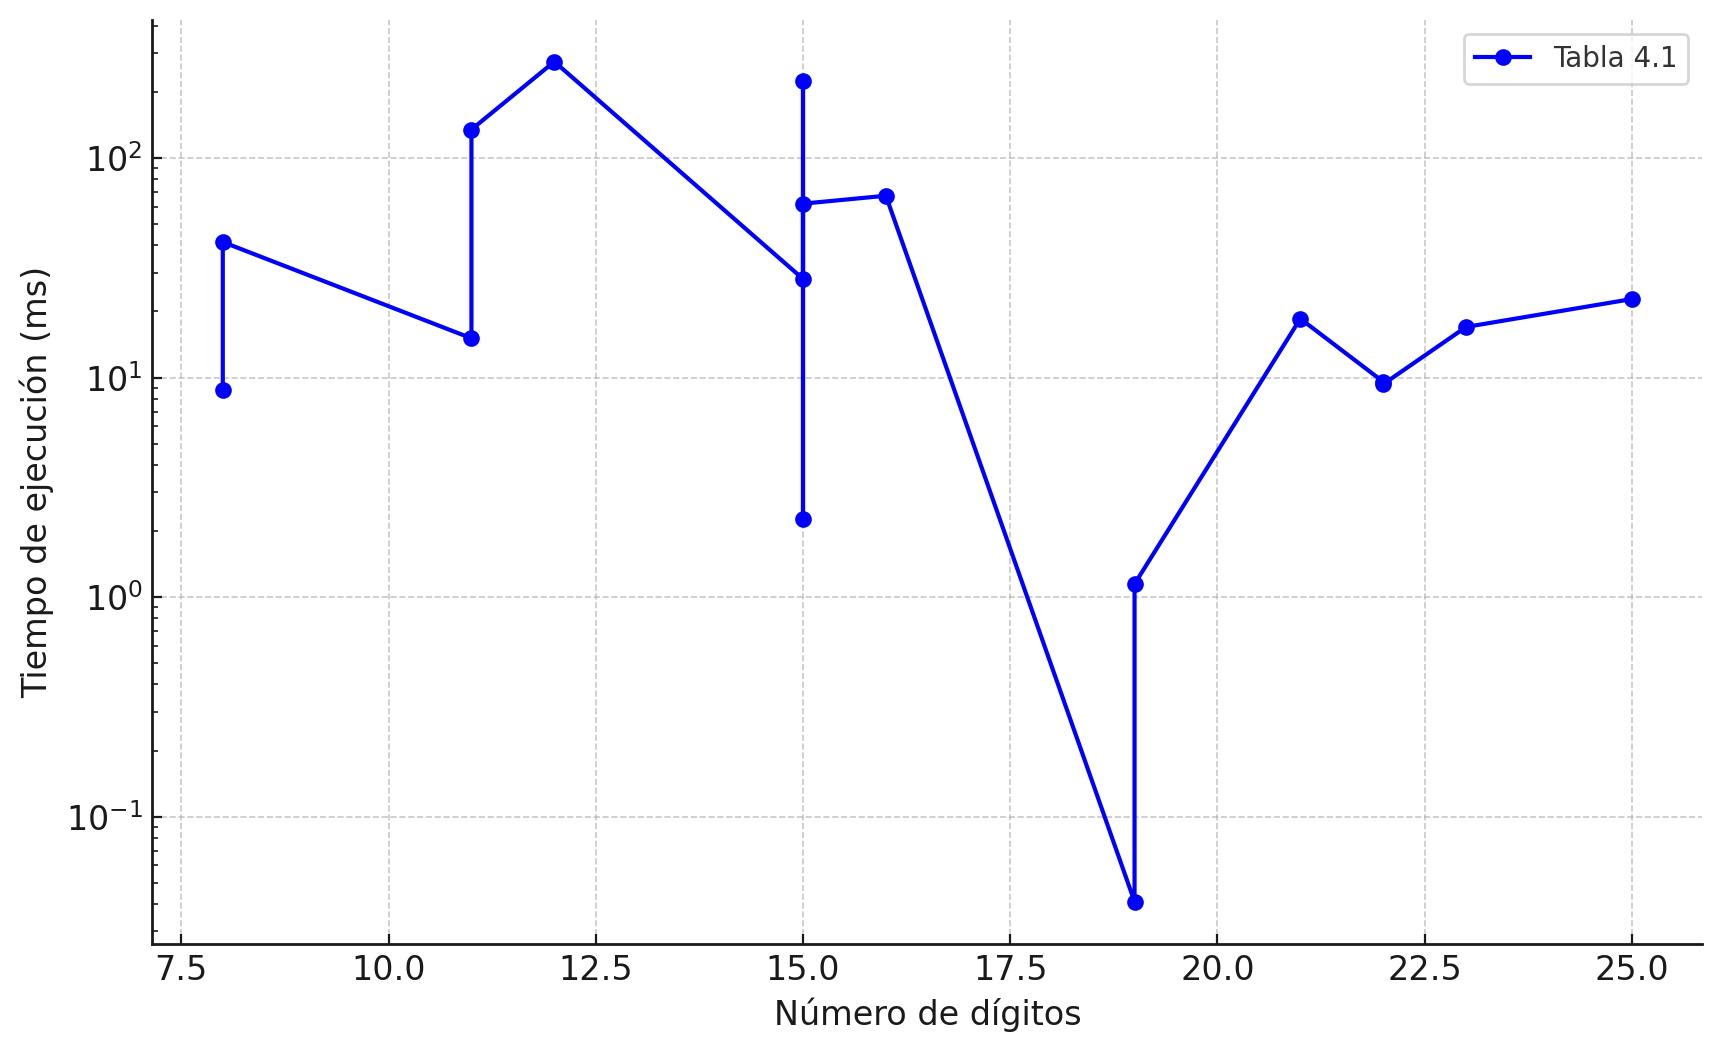
\includegraphics[width=\linewidth]{images/res-curva-eliptica.png}
        \caption{Resultados Método de Factorización con Curvas Elípticas con casos de prueba de la Tabla \ref{tabla:factores_pequeños}}
    \end{figure}

    \subsection{ALGORITMO DE FACTORIZACIÓN DE CRIBA CUADRÁTICA}
    El método de factorización de Criba Cuadrática tiene una complejidad temporal de \\ $O(e^{(1+o(n))\sqrt{\log n \log \log n}})$ en el peor caso.

    Para este algoritmo se usaran los casos de prueba de la Tabla \ref{tabla:factores_mitad} y Tabla \ref{tabla:primos_cercanos}
    \begin{table}[H]
        \centering
        \begin{tabular}{ccc}
        \toprule
        Número a factorizar & Tiempo de ejecución (ms) & Factores primos encontrados\\
        \midrule
        16236991 & 84.607 & [4831.0, 3361.0]\\
        469526207 & 51.509 & [25261.0, 18587.0]\\
        914465141 & 76.737 & [44111, 20731]\\
        45774604399 & 84.415 & [216743.0, 211193.0]\\
        138426627499 & 97.567 & [225343, 614293]\\
        2002311773621 & 92.401 & [703709, 2845369]\\
        36162913278367 & 99.894 & [4352419, 8308693]\\
        279747589361921 & 103.140 & [29908387, 9353483]\\
        3064287451898711 & 95.126 & [38873827, 78826493]\\
        6587155271801233 & 108.067 & [101689751, 64776983]\\

        \bottomrule
        \end{tabular}
        \caption{Resultados de la Factorización por Criba Cuadrática para los casos de prueba de la Tabla \ref{tabla:factores_mitad}}
        \label{tab:res-qs-mitad}
    \end{table}

    \begin{table}[H]
        \centering
        \begin{tabular}{ccc}
        \toprule
        Número a factorizar & Tiempo de ejecución (ms) & Factores primos encontrados\\
        \midrule
        66436879 & 69.424 & [8287.0, 8017.0]\\
        686703811 & 70.688 & [26431.0, 25981.0]\\
        8101438039 & 70.603 & [90053.0, 89963.0]\\
        85526931211 & 74.497 & [292717.0, 292183.0]\\
        262209534767 & 57.068 & [512137.0, 511991.0]\\
        715281207649 & 90.008 & [845863.0, 845623.0]\\
        1873966393597 & 82.297 & [1369391.0, 1368467.0]\\
        18701749916023 & 69.058 & [4324843.0, 4324261.0]\\
        1757788889012333 & 68.385 & [41926147.0, 41925839.0]\\
        \bottomrule
        \end{tabular}
        \caption{Resultados de la Factorización por Criba Cuadrática para los casos de prueba de la Tabla \ref{tabla:primos_cercanos}}
        \label{tab:res-qs-cercano}
    \end{table}

    \begin{figure}[H]
        \centering
        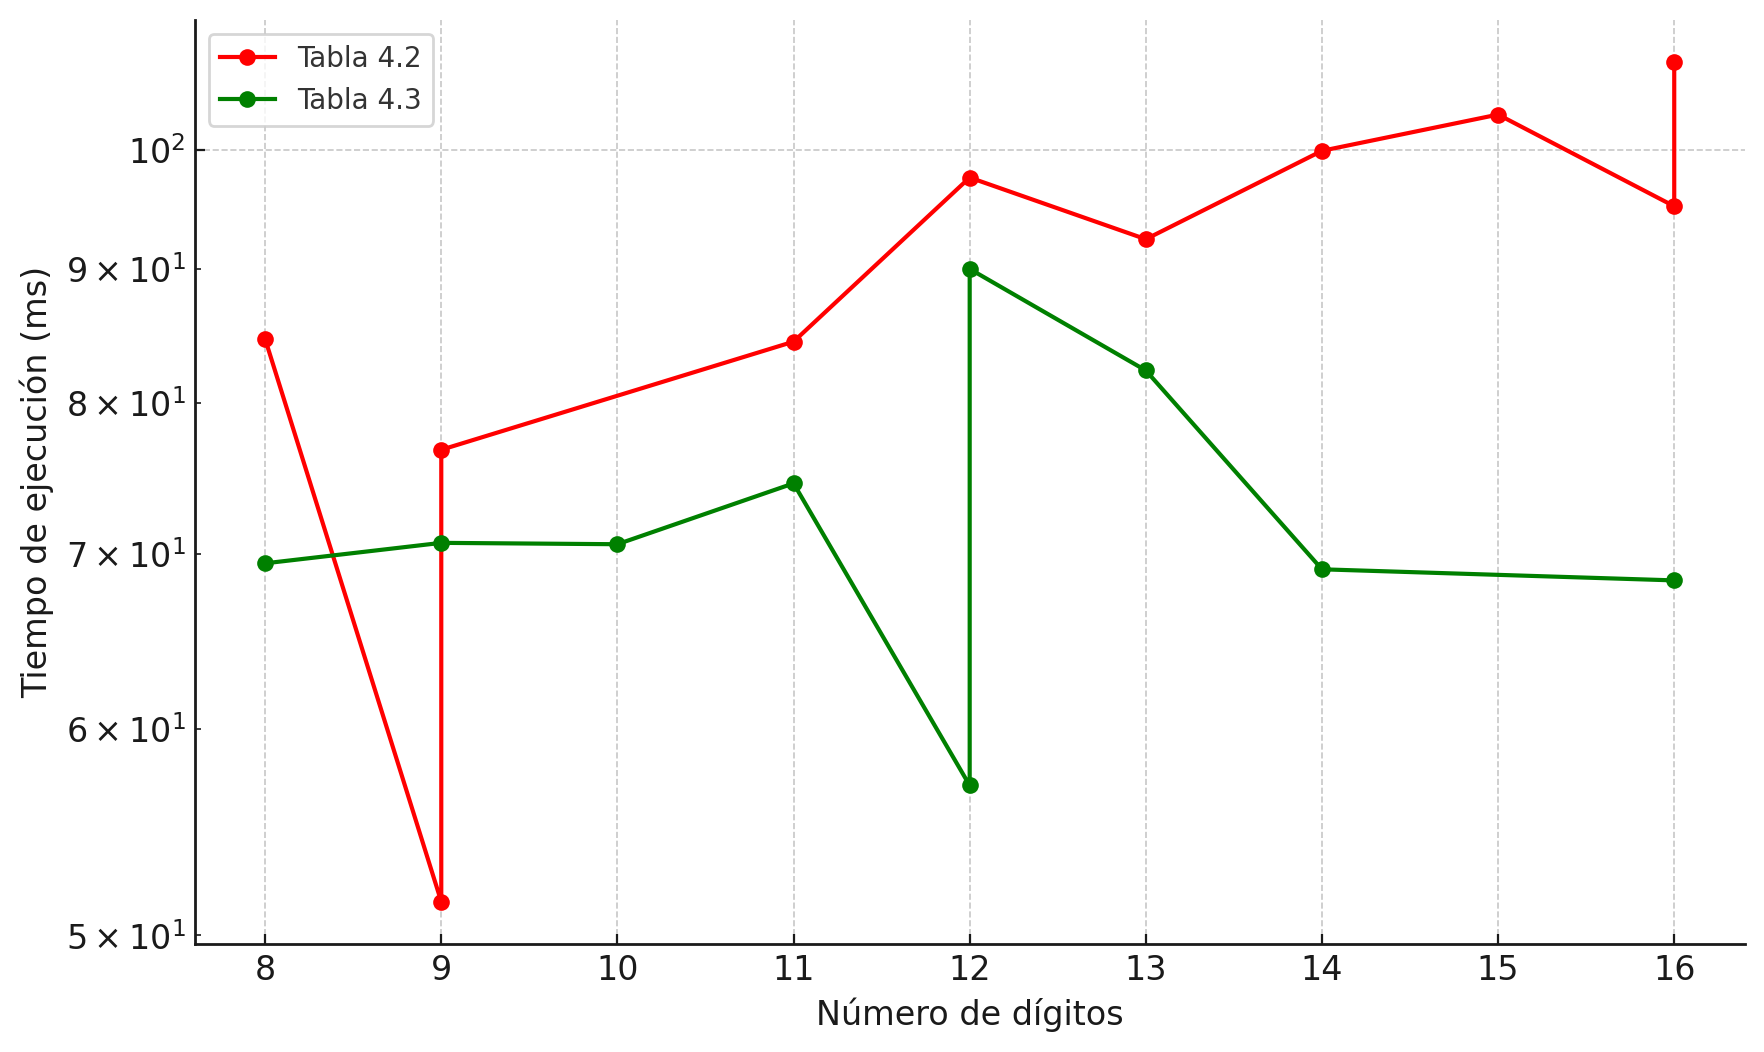
\includegraphics[width=\linewidth]{images/res-qs.png}
        \caption{Resultados la Factorización con Criba Cuadrática}
    \end{figure}

    % \subsection{MÉTODO DE FACTORIZACIÓN CON FRACCIONES CONTINUAS}
    % El método de factorización con Fracciones Continuas tiene una complejidad temporal de $O((\log n)^2)$ en el peor caso y una complejidad espacial de $O(\log n)$.

    \section{DEMOSTRACIÓN DE LA HIPÓTESIS}
    Para la demostración de la hipótesis se hará uso de los resultados obtenidos en las comparaciones, observando el tiempo de ejecución, el espacio de memoria utilizado y los factores primos encontrados.

    Para la prueba de hipotesis utilizaremos los resultados de los diferentes algoritmos con los casos de prueba de la Tabla \ref{tabla:primos_cercanos}.

    \begin{table}[H]
        \centering
        \begin{adjustbox}{width=\columnwidth,center}
        \begin{tabular}{|c|c|c|c|c|}
        \hline
        Número a factorizar & Divisiones Sucesivas & Fermat & Pollard Rho & Criba Cuadrática\\ \hline
        66436879        & 0.437                  & 0.009                  & 0.213                  & 69.424                 \\ \hline
        686703811       & 1.394                  & 0.03                   & 0.235                  & 70.688                 \\ \hline
        8101438039      & 6.293                  & 0.036                  & 0.28                   & 70.603                 \\ \hline
        85526931211     & 21.026                 & 0.003                  & 2.49                   & 74.497                 \\ \hline
        262209534767    & 39.504                 & 0.002                  & 1.729                  & 57.068                 \\ \hline
        715281207649    & 64.788                 & 0.002                  & 1.384                  & 90.008                 \\ \hline
        1873966393597   & 109.328                & 0.002                  & 1.494                  & 82.297                 \\ \hline
        18701749916023  & 339.266                & 0.002                  & 0.481                  & 69.058                 \\ \hline
        1757788889012333 & 3414.5                & 0.002                  & 15.424                 & 68.385                 \\ \hline
        34843998810184129 & 15096.03             & 0.002                  & 14.593                 &   103.500                     \\ \hline
        874655409151893869 & 81195.058           & 0.002                  & 62.654                 &  84.799                      \\ \hline
        286073409635796583 & 43553.943           & 0.002                  & 11.13                  &  88.860                      \\ \hline
        \end{tabular}
        \end{adjustbox}
        \caption{Tiempos de ejecución para diferentes algoritmos con los casos de prueba de la Tabla \ref{tabla:primos_cercanos}}
        \label{tabla:tiempos}
    \end{table}

    Comparación entre Divisiones Sucesivas y Algoritmo de Fermat:
    \[
        \text{Estadístico t: } 1.6454
    \]
    \[
        \text{Valor p: } 0.1281
    \]
    No se rechaza la hipótesis nula: no hay una diferencia significativa entre los algoritmos.


    Comparación entre Divisiones Sucesivas y Algoritmo Pollard-Rho
    \[
        \text{Estadístico t: } 1.6452
    \]
    \[
        \text{Valor p: } 0.1282
    \]
    No se rechaza la hipótesis nula: no hay una diferencia significativa entre los algoritmos.

    Comparación entre Divisiones Sucesivas y Criba Cuadratica
    \[
        \text{Estadístico t: } 1.6352
    \]
    \[
        \text{Valor p: } 0.1303
    \]
    No se rechaza la hipótesis nula: no hay una diferencia significativa entre los algoritmos.

    Comparación entre Algoritmo de Fermat y Algoritmo Pollard-Rho
    \[
        \text{Estadístico t: } -1.8211
    \]
    \[
        \text{Valor p: } 0.0959
    \]
    No se rechaza la hipótesis nula: no hay una diferencia significativa entre los algoritmos.

    Comparación entre Algoritmo de Fermat y Criba Cuadratica
    \[
        \text{Estadístico t: } -21.0917
    \]
    \[
        \text{Valor p: } 0.0000
    \]
    Rechazamos la hipótesis nula: hay una diferencia significativa entre los algoritmos.

    Comparación entre Algoritmo Pollard-Rho y Criba Cuadratica
    \[
        \text{Estadístico t: } -12.9675
    \]
    \[
        \text{Valor p: } 0.0000
    \]
    Rechazamos la hipótesis nula: hay una diferencia significativa entre los algoritmos.

    \clearpage
\chapter{CONCLUSIONES Y RECOMENDACIONES}

\section{CONCLUSIONES}
El algoritmo de Fermat, es el más rápido cuando la diferencia entre los factores primos es pequeña y en este campo es superior a los demás algoritmos.

Si se desea factorizar números que tengan factores primos pequeños, el algoritmo de divisiones sucesivas puede ser utilizado y tiene una complejidad muy baja en cuanto a su implementación.

El algoritmo de Pollard Rho es el algoritmo predilecto para uso general en cuanto se trate de factorizar números de uso cotidiano, por la complejidad que aporta y los factores primos encontrados.

Mientras que si se desea trabajar en el campo de la criptografía o un uso más especializado en el area de Teoría De números el mejor algoritmo en estos casos es la Criba General de Cuerpo de Números o la Criba Cuadrática, estos algoritmos requieren de una comprensión más profunda de la parte teórica y una correcta implementación para su uso adecuado.

\section{RECOMENDACIONES}
Una vez concluido el presente trabajo se sugiere la posibilidad de continuar con algunas de las líneas de investigación desarrolladas e incluso incursionar en otras relacionadas con los temas tratados, se recomienda seguir con las siguientes temáticas.

Continuar con el estudio de los algoritmos cuánticos y algoritmos híbridos para posibles avances en el area de criptografía.
    \clearpage
% \chapter{BIBLIOGRAFÍA}
\addcontentsline{toc}{chapter}{BIBLIOGRAFÍA}
\printbibliography

    \counterwithin{figure}{chapter}
    % \endgroup
    % \bibliographystyle{apacite}
    % \bibliography{capitulos/biblio.bib}
	%--------------------------------------------------
	
	
	
	%BACKMATTER
	%---------------------------------------------------
% 	\backmatter
% 	%BIBLIOGRAFÍA.
% 	%\cleardoublepage
% 	\addcontentsline{toc}{chapter}{Bibliografía}
% 	\bibliographystyle{apalike}
% 		\bibliography{capitulos/biblio}
		
%---------------------------------------------------	
	
\end{document}
